%% =======================================================================================
%% 
%% RELATÓRIO TÉCNICO
%% Criado a partir da classe abntex2, desenvolvida pelo 
%% Centro de Pesquisa em Arquitetura da Informação (CPAI)
%% 
%% Arquivos de dados:   sty/configs.sty         % Configuração dos pacotes LaTeX
%%                      sty/metadados_rt.sty    % METADADOS DO RELATÓRIO - PREENCHER!
%%                      sty/dados_cpai.sty      % Informações institucionais CPAI / FUB
%%                      sty/timbrado.sty        % Formatação do documento (layout)
%%                      sty/vocabulario.sty     % Comandos LaTeX para facilitar digitação
%% 
%% =======================================================================================

\documentclass[pdftex,11pt,oneside,a4paper,english,italian,spanish,brazil]{abntex2}


% ----------------------------------------------------------------------------------------
% - PACOTES
  \usepackage{sty/configs}                  % Pacotes utilizados
  \usepackage{sty/metadados_rt}             % Dados do órgão / cliente
  \usepackage{sty/dados_cpai}               % Dados do CPAI/FUB
  \usepackage{sty/vocabulario}              % Vocabulário específico do projeto
  \usepackage{sty/leiaute_rt} 
  \usepackage{caption} 
  \renewcommand\captionfont{\footnotesize} 

  \usepackage{listings} 
%\lstset{emph={trueIndex,root},emphstyle=\color{BlueViolet}}%\underbar} % For special keywords
\lstset{language=[LaTeX]Tex,%C++ % Specify the language(s) for listings here
morekeywords={PassOptionsToPackage,selectlanguage},
keywordstyle=\color{RoyalBlue}, % Add \bfseries for bold
basicstyle=\small\ttfamily, % Makes listings a smaller font size and a different font
%identifierstyle=\color{NavyBlue}, % Color of text inside brackets
commentstyle=\color{Green}\ttfamily, % Color of comments
stringstyle=\rmfamily, % Font type to use for strings
numbers=left, % Change left to none to remove line numbers
numberstyle=\scriptsize, % Font size of the line numbers
stepnumber=5, % Increment of line numbers
numbersep=8pt, % Distance of line numbers from code listing
showstringspaces=false, % Sets whether spaces in strings should appear underlined
breaklines=true, % Force the code to stay in the confines of the listing box
%frameround=ftff, % Uncomment for rounded frame
%frame=single, % Frame border - none/leftline/topline/bottomline/lines/single/shadowbox/L
belowcaptionskip=.75\baselineskip % Space after the "Listing #: Desciption" text and the listing box
}            % Definições de layout do documento
\usepackage{xcolor}
\lstset{
   basicstyle=\fontsize{9}{9}\selectfont\ttfamily,
frame=lrb,xleftmargin=\fboxsep,xrightmargin=-\fboxsep}
\DeclareCaptionFont{white}{\color{white}}
\DeclareCaptionFormat{listing}{%
  \parbox{\textwidth}{\colorbox{gray}{\parbox{\textwidth}{#1#2#3}}\vskip-0pt}}
\captionsetup[lstlisting]{format=listing,labelfont=white,textfont=white}
% ----------------------------------------------------------------------------------------
\renewcommand{\lstlistingname}{Listato}
% ----------------------------------------------------------------------------------------
% - INÍCIO DO DOCUMENTO
  \begin{document}
      \begin{sloppypar}
          
          % Seleciona o idioma do documento (conforme pacotes do babel)
            %\selectlanguage{english}
            \selectlanguage{italian}
            
          % Retira espaço extra obsoleto entre as frases.
            \frenchspacing
          
          % ------------------------------------------------------------------------------
          % - ESTRUTURA DO DOCUMENTO
          % ------------------------------------------------------------------------------
          % ------------------------------------------------------------------------------
          % - PRÉ-TEXTUAL
          % ------------------------------------------------------------------------------
          \pretextual

          % Capa
            %~~~~~~~~~~~~~~~~~~~~~~~~~~~~~~~~~~~~~~~~~~~~~~~~~~~~~~~~~~~~~~~~~~~~~
% File  : capa
%~~~~~~~~~~~~~~~~~~~~~~~~~~~~~~~~~~~~~~~~~~~~~~~~~~~~~~~~~~~~~~~~~~~~~

  \thispagestyle{empty}

  \ThisCenterWallPaper{1}{img/dieti_wall.png}

  \begin{flushright}

    \begin{minipage}{0.6\textwidth}
      \begin{flushleft}
          \sffamily
          % Parte superior da capa
          \vspace{2cm}
          \normalsize Corso di Laurea Magistrale in \\\Large Ingegneria Informatica \\
          \footnotesize \textcolor{black!60}{} \\[2cm]
          \begin{center}
          	
          \end{center}
          \large Elaborato del corso di \Large \textit{Applicazioni Telematiche}\\
          \HUGE Secure Messaging\\
          \large Documentazione
      \end{flushleft}
    \end{minipage}%

    \vfill
    \begin{minipage}{0.6\textwidth}
       % \begin{center}
          \sffamily
          \small \textit{Parricelli Francesco} M63/720 \\
          \textit{Strofaldi Aldo} M63/728\\
          \textit{Pirozzi Luca} M63/744\\
          
          Anno Accademico 2017/2018\\
       % \end{center}
    \end{minipage}%
  \end{flushright}

            \cleardoublepage
          
          \shipout \null

          % Sumarios
            \vspace{1cm}
            
   
            \tableofcontents
            
          % Lista de abreviaturas e siglas
         
            
          % ------------------------------------------------------------------------------
          % - TEXTUAL
          % ------------------------------------------------------------------------------
          %%Inserire qui capitoli
          %~~~~~~~~~~~~~~~~~~~~~~~~~~~~~~~~~~~~~~~~~~~~~~~~~~~~~~~~~~~~~~~~~~~~~
%    File      : webanalysis
%~~~~~~~~~~~~~~~~~~~~~~~~~~~~~~~~~~~~~~~~~~~~~~~~~~~~~~~~~~~~~~~~~~~~~


\label{cap:dependability}

%~~~~~~~~~~~~~~~~~~~~~~~~~~~~~~~~~~~~~~~~~~~~~~~~~~~~~~~~~~~~~~~~~~~~~
%    File      : webanalysis
%~~~~~~~~~~~~~~~~~~~~~~~~~~~~~~~~~~~~~~~~~~~~~~~~~~~~~~~~~~~~~~~~~~~~~
\textual 

\chapter{Introduzione}


Secure Messaging, elaborato del corso di Applicazioni Telematiche, è un'applicazione per la messaggistica sicura, in grado cioè di garantire confidenzialità, integrità e autenticità (mediante protocollo di trasporto DTLS), sviluppata cercando di renderla il più possibile simile ad una reale.
 
L'applicazione è strutturata secondo l'architettura Client/Server: nello specifico il Web Server utilizzato è stato Apache Tomcat, contenente Java Servlet, un modulo NodeJS (con supporto WebSocket) per la gestione della segnalazione  mentre il client è di tipo web, sviluppato facendo uso di HTML, Javascript/JQuery e AJAX, CSS.
Si è inoltre fatto uso di altre tecnologie e linguaggi come ad esempio XACML per il controllo accessi, JSON/XML come formato di interscambio dati (con l'utilizzo delle API JAXB per la manipolazione XML), HTTPS per la comunicazione sicura client/server (sia per il server Tomcat, sia per il server NodeJS), SQL per il database.

Di seguito si definisce e si illustra uno schema di massima astrazione, atto a concepire da un'ottica di alto livello, il funzionamento del sistema.

\begin{figure}[!htbp]
	\centering
	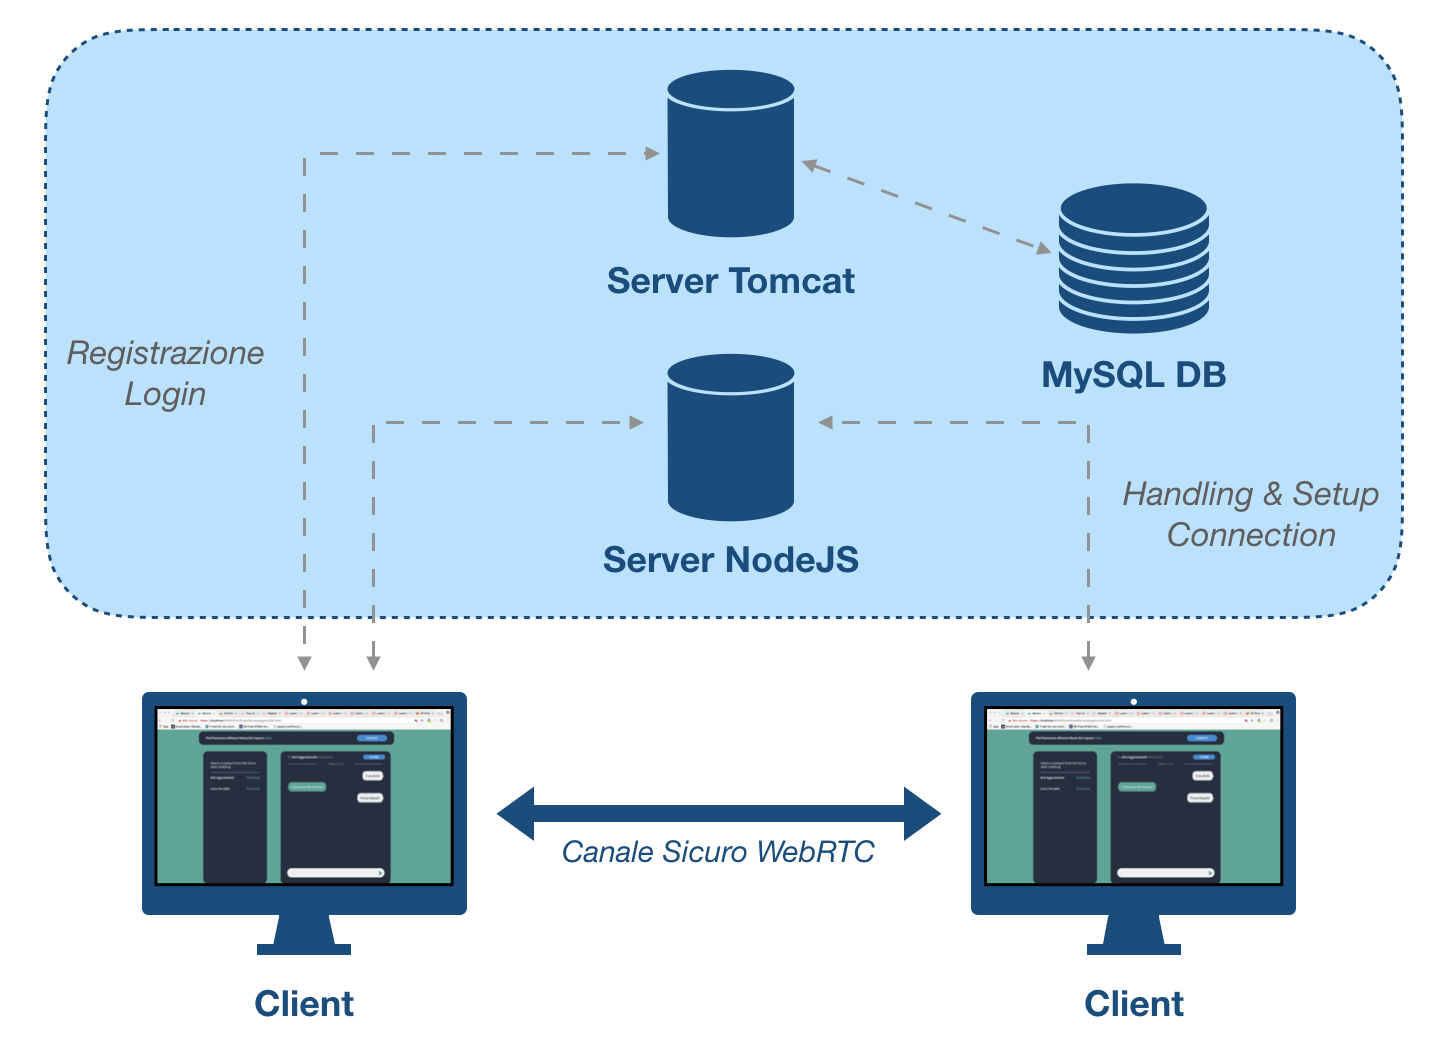
\includegraphics[scale = .6]{img/schemaGenerale}
	\caption{Schema di alto livello dell'applicazione}
	\label{gfx:schemaGenerale}
\end{figure}

Oltre a implementatare la comunicazione crittografata end-to-end facendo uso di WebRTC così come da specifica , sono stati introdotti ulteriori meccanismi che ci aspetteremmo di trovare solo in sistemi effettivamente rilasciati sul mercato: ciò risulta essere il risultato di un percorso di studi che ci ha portato a considerare lo sviluppo di un sistema software o embedded come qualcosa che vada oltre la semplice considerazione di correttezza e prestazioni, ma che include anche altri fattori come robustezza, confidenzialità e integrità.

Tenendo sempre in considerazione i vincoli di tempo e di sviluppatori, sono stati affrontati problemi tipici di applicazioni reali come ad esempio la protezione dell'account, che si è tradotta nella limitazione dei tentativi di accesso all'account (fino al blocco IP) per dispositivo, in modo da frustrare tentativi di attacchi brute-force e autenticazione a due passi. Le password, così come dalle linee guida di numerose organizzazioni, sono state criptate (con salt autogenerato) mediante algoritmo bCrypt. Le richieste contengono token che sono limitati nel numero di utilizzi, caratterizzati da un timestamp (e relativa scadenza), associati ad un IP e firmati dal server per evitare attacchi comuni come il replay attack.\\
Sono state inoltre seguite le direttive \textit{OWASP} per la mitigazione degli attacchi XSS (Cross-Site Scripting) mediante l'utilizzo di \textit{Content Security Policy} (CSP) headers.

Uno sguardo attento è stato rivolto alla considerazione di ogni scenario possibile facendo uso del client web, cercando di garantire che i dati immessi dall'utente siano sempre ben formati alla sorgente (mail, campi numerici, ecc.), garantendo robustezza e alleggerendo il carico del server e riducendo le possibilità di richieste mal costruite ed errori. Un esempio è l'utilizzo di regex per il controllo della validità di una mail.

In termini pratici, l'applicazione consente lo scambio di messaggi tra utenti in maniera sicura. Non tutti gli utenti sono abilitati a scambiarsi messaggi, ma ciò è possibile solo rispetto alle politiche XACML implementate:
\begin{enumerate}
	\item Gli utenti possono richiedere una sessione solo con i tecnici;
	\item I tecnici possono richiedere una sessione con altri tecnici o con utenti;
	\item Gli amministratori possono richiedere una sessione con i tecnici, utenti e altri amministratori.
	\end{enumerate}
\newpage
\chapter{Documentazione}
%~~~~~~~~~~~~~~~~~~~~~~~~~~~~~~~~~~~~~~~~~~~~~~~~~~~~~~~~~~~~~~~~~~~~~
%    File      : webanalysis
%~~~~~~~~~~~~~~~~~~~~~~~~~~~~~~~~~~~~~~~~~~~~~~~~~~~~~~~~~~~~~~~~~~~~~

\textual

%\chapter{Dependability}\label{cap:dependability}

\section{Documentazione Server Tomcat}

In questa sezione vengono mostrati i diagrammi UML relativamente alla realizzazione del Server Tomcat, su cui sono installate le Servlet per la gestione delle politiche di login e registrazione, nonché l'interfacciamento con la base di dati e con il mail server.

\subsection{Diagramma delle Classi}

Di seguito viene riportato il diagramma delle classi di Secure Messaging: piuttosto che limitarci ad allegare un solo diagramma, troppo complesso e poco informativo, si riportano le classi per package e relazioni intra ed inter-package; in questo modo abbiamo suddiviso il diagramma delle classi originali in porzioni sufficientemente piccole da poter essere analizzate con profitto ma sufficientemente grandi da essere significative, che nell’insieme permette ad un programmatore la giusta documentazione per individuare struttura e dipendenza delle classi con l’adeguata granularità di informazioni.
Per ragioni di semplicità sono state omesse le relazioni al package delle eccezioni, da cui praticamente tutti i package dipendono.

\subsubsection{Package: \textbf{access control}}

Contiene la classe che si occupa delle operazioni per prevenire o individuare le intrusioni in un account, aggiornare i conteggi dei login falliti e bloccare i tentativi di accesso.

\begin{figure}[!htbp]
	\centering
	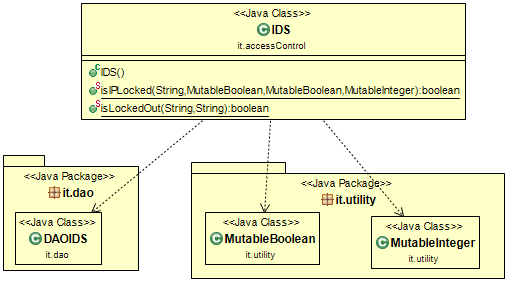
\includegraphics[scale = .6]{img/dependencies_accesscontrol.png}
	\caption{Package Access Control}
	\label{gfx:accesscontrol}
\end{figure}


\subsubsection{Package: \textbf{authentication}}

Appartengono a questo package la servlet di autenticazione e la relativa logica (disaccoppiata dalla servlet per il principio della separazione degli interessi). Il package è visualizzato in figura \ref{gfx:dependencies_authentication}.

\tiny 
\begin{landscape}
\begin{center}
\vspace*{\fill}
\begin{figure}[!htbp]
	\centering
	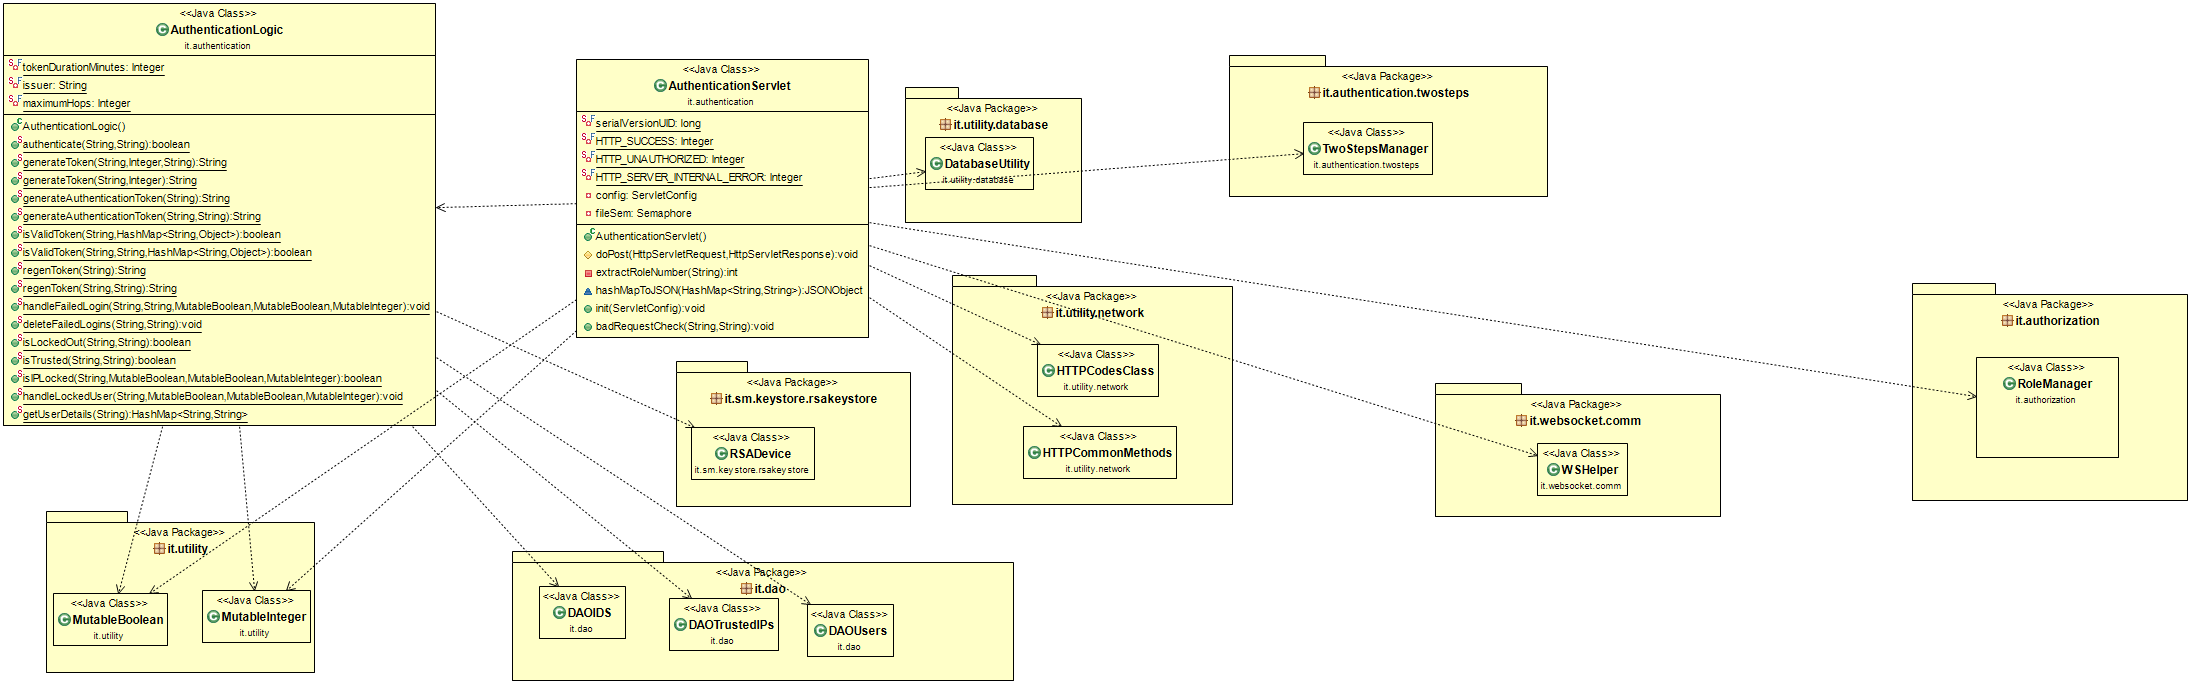
\includegraphics[scale = .3]{img/dependencies_authentication}
	\caption{Package Authentication}
	\label{gfx:dependencies_authentication}
\end{figure}
\vspace*{\fill}

\end{center}	

\end{landscape}%
\normalsize

\subsubsection{Package: \textbf{authorization}}

Le classi di questo package si occupano di determinare se l’utente è autorizzato ad effettuare una determinata operazione.\\
In particolare, contiene un filtro (ContactListFilter) che si occupa di filtrare le richieste che vengono fatte verso le diverse contact-lists disponibili, ed accettarle in base al rispetto delle policy XACML previste.

Il package è visualizzato in figura \ref{gfx:dependencies_authorization}.

\begin{figure}[!htbp]
	\centering
	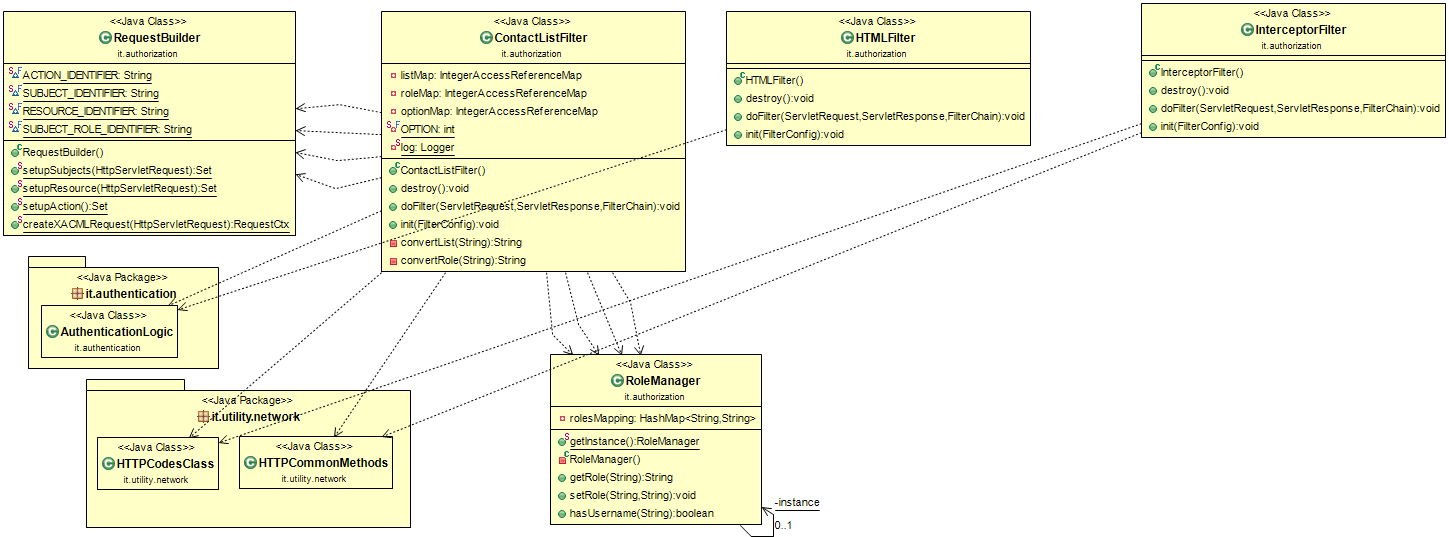
\includegraphics[scale = .3]{img/dependencies_authorization}
	\caption{Package Authorization}
	\label{gfx:dependencies_authorization}
\end{figure}

\subsubsection{Package: \textbf{bcrypt}}

Package importato da una libreria OTS che implementa hashing/salting delle password con algoritmo bcrypt (utilizzato, fra gli altri, da OpenBSD). 
Il package è visualizzato in figura \ref{gfx:dependencies_bcrypt}.

\begin{figure}[!htbp]
	\centering
	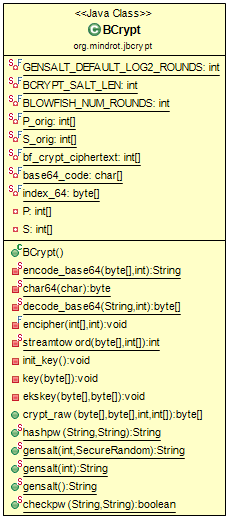
\includegraphics[scale = .5]{img/dependencies_bcrypt}
	\caption{Package BCrypt}
	\label{gfx:dependencies_bcrypt}
\end{figure}

\subsubsection{Package: \textbf{DAO}}

Questo package rappresenta il ponte tra i dati del database e l’applicazione. Sono le classi a cui le altre si rivolgono per operare su dati che altrimenti sarebbero da prelevare direttamente dal database. 

Il package è visualizzato in figura \ref{gfx:dependencies_dao}.

\begin{figure}[!htbp]
	\centering
	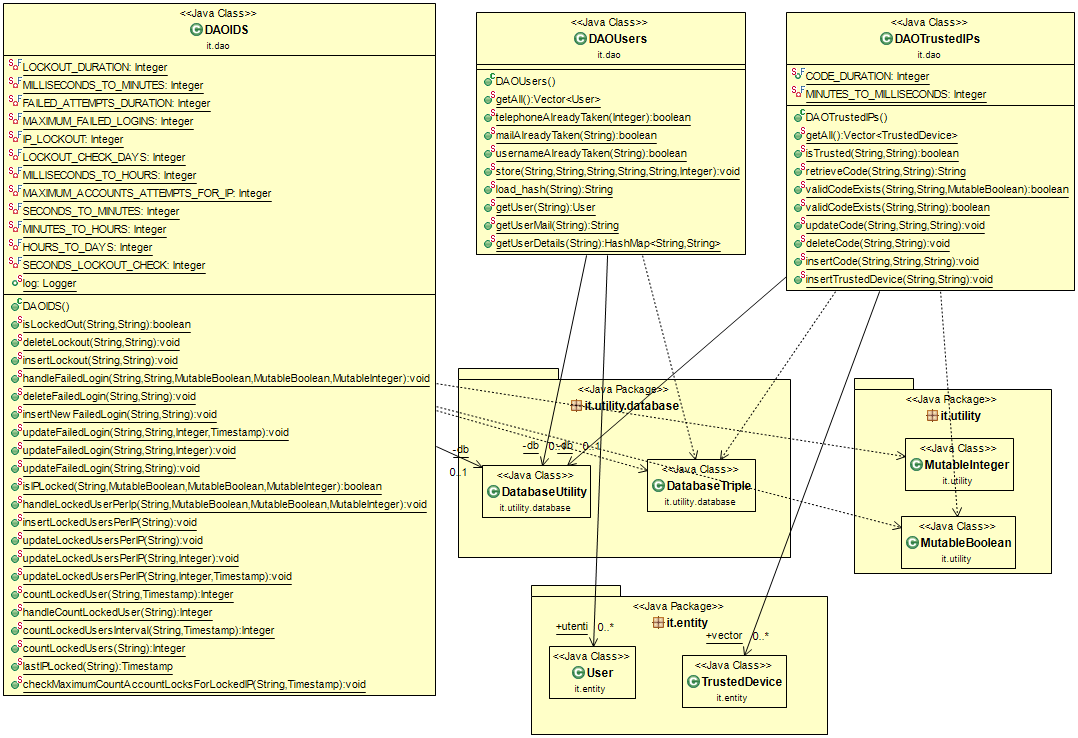
\includegraphics[scale = .4]{img/dependencies_dao}
	\caption{Package DAO}
	\label{gfx:dependencies_dao}
\end{figure}

\subsubsection{Package: \textbf{entity}}

Costituiscono una rappresentazione Object-oriented che effettua il mapping rispetto alla rappresentazione del db.

Il package è visualizzato in figura \ref{gfx:dependencies_entity}.

\begin{figure}[!htbp]
	\centering
	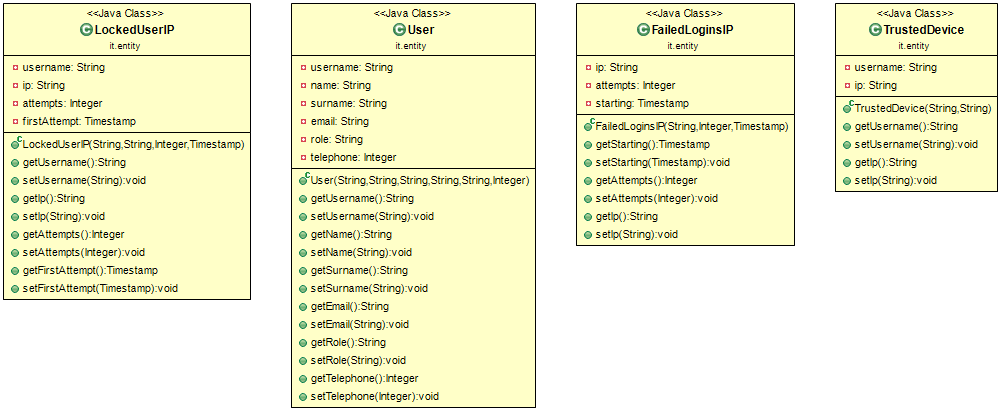
\includegraphics[scale = .4]{img/dependencies_entity}
	\caption{Package Entity}
	\label{gfx:dependencies_entity}
\end{figure}

\subsubsection{Package: \textbf{exception}}

Raccoglie tutte le eccezioni che possono essere lanciate. A sua volta è diviso in sotto-package che non vengono rappresentati per semplicità.

Il package è visualizzato in figura \ref{gfx:dependencies_exception}, a pagina successiva.

\tiny 
\begin{landscape}
\begin{center}
\vspace*{\fill}
\begin{figure}[!htbp]
	\centering
	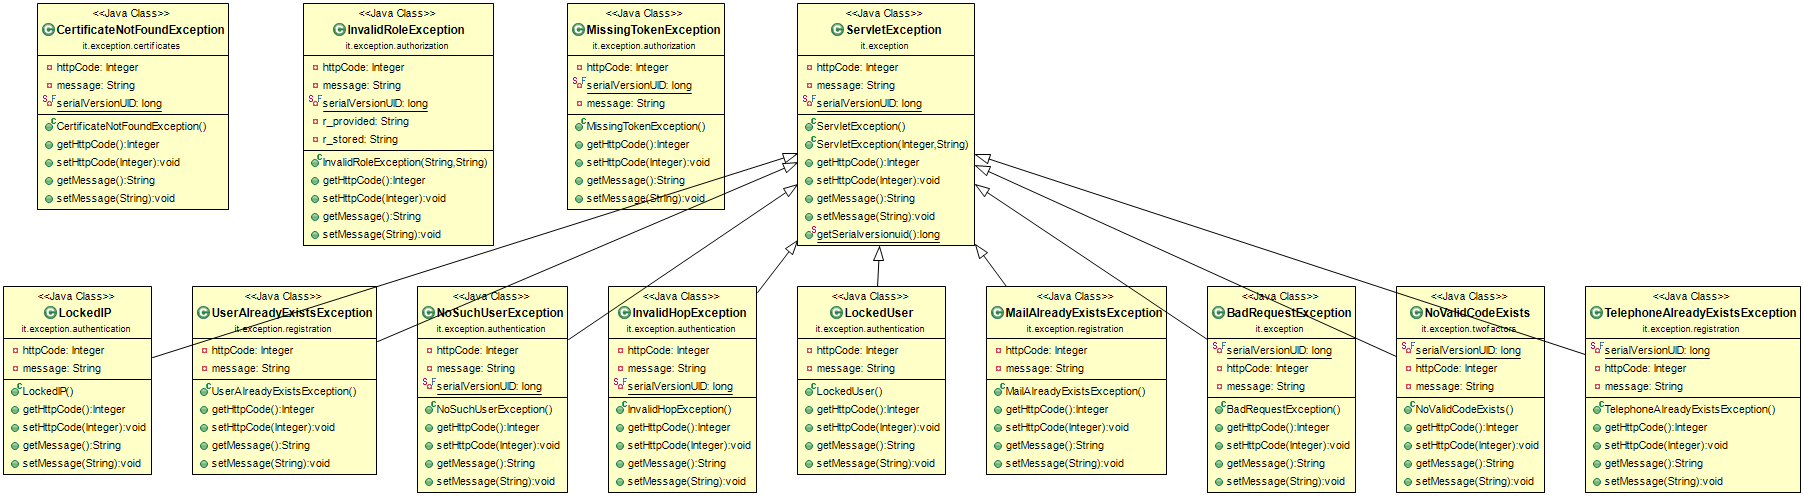
\includegraphics[scale = .3]{img/dependencies_exception}
	\caption{Package Exception}
	\label{gfx:dependencies_exception}
\end{figure}
\vspace*{\fill}

\end{center}	

\end{landscape}%
\normalsize
\subsubsection{Package: \textbf{keystore}}

Contiene la semplice interfaccia che ci aspetteremmo da un’entità crittografica: la capacità di criptare e decriptare bytes. Implementeranno l’interfaccia tutte quelle classi che si occuperanno di crittografare dati (implementando gli specifici algoritmi di cui MyKeystore è indipendente).

Il package è visualizzato in figura \ref{gfx:dependencies_keystore}.

\begin{figure}[!htbp]
	\centering
	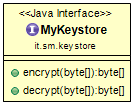
\includegraphics[scale = .5]{img/dependencies_keystore}
	\caption{Package Keystore}
	\label{gfx:dependencies_keystore}
\end{figure}

\subsubsection{Package: \textbf{keystore.rsaKeystore}}

Package innestato nel precedente che rappresenta una crittografia specifica, in questo caso di tipo RSA. Simula le caratteristiche di una smart-card (di cui avremmo bisogno per una criptografia sicura) in software, e usa le chiavi private e pubblica per codificare e decodificare: la privata viene usate per codificare i dati da mandare al client, la pubblica quelli che solo il server può leggere, come la chiave AES utilizzata per codificare i parametri di accesso al db e al mail server.


Il package è visualizzato in figura \ref{gfx:keystore.rsaKeystore}.

\begin{figure}[!htbp]
	\centering
	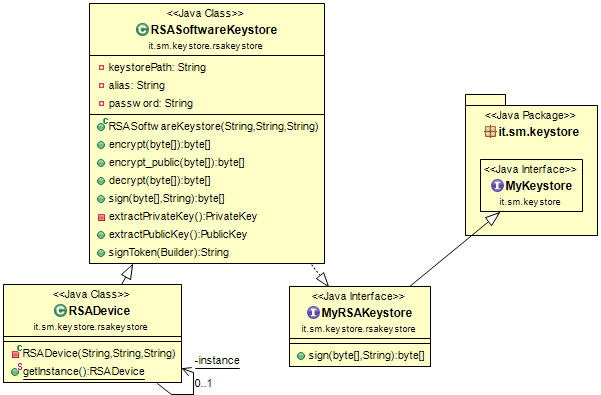
\includegraphics[scale = .5]{img/dependencies_rsakeystore.png}
	\caption{Package keystore.rsaKeystore}
	\label{gfx:keystore.rsaKeystore}
\end{figure}

\subsubsection{Package: \textbf{registration}}

Appartengono a questo package la servlet e la logica di registrazione.


Il package è visualizzato in figura \ref{gfx:registration}.

\begin{figure}[!htbp]
	\centering
	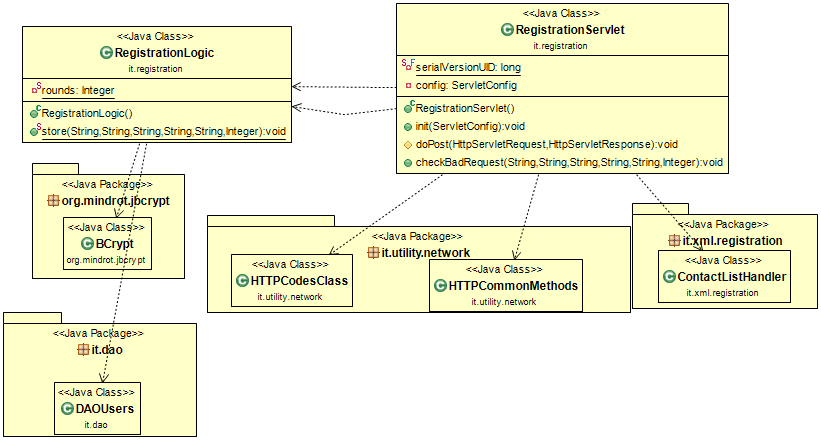
\includegraphics[scale = .5]{img/dependencies_registration.png}
	\caption{Package Registration}
	\label{gfx:registration}
\end{figure}


\subsubsection{Package: \textbf{twosteps}}

Di questo package fanno parte le classi che si occupano dell’autenticazione in due passi; la classe TwoStepsServlet rappresenta la servlet a cui rivolgersi per l’invio del codice, ed effettua chiamate a TwoStepsLogic per ciò che concerne la logica delle operazioni, mentre TwoStepsManager si occupa dell’invio della mail nel caso in cui fosse richiesta.

Il package è visualizzato in figura \ref{gfx:dependencies_twosteps}.

\begin{figure}[!htbp]
	\centering
	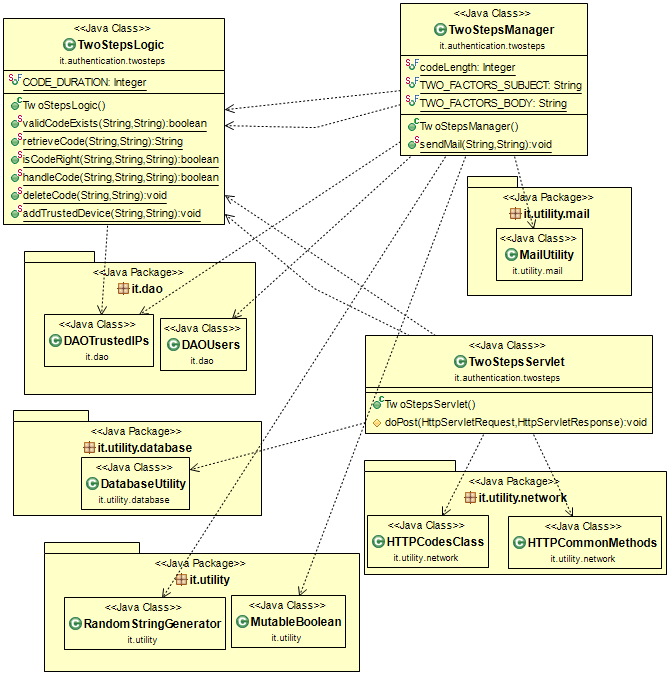
\includegraphics[scale = .5]{img/dependencies_twosteps.png}
	\caption{Package Twosteps}
	\label{gfx:dependencies_twosteps}
\end{figure}

\subsubsection{Package: \textbf{utility}}

Contiene diverse classi di utilità, utilizzate per risolvere in modo semplice alcuni semplici compiti, come la generazione del codice per l’autenticazione a due step (RandomStringGenerator).


Il package è visualizzato in figura \ref{gfx:dependencies_utility}.

\begin{figure}[!htbp]
	\centering
	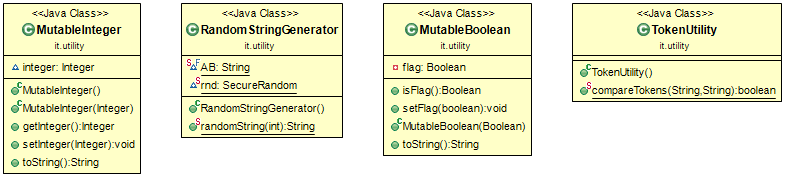
\includegraphics[scale = .5]{img/dependencies_utility}
	\caption{Package Utility}
	\label{gfx:dependencies_utility}
\end{figure}

\subsubsection{Package: \textbf{utility.database}}

A questo package appartengono delle classi di utilità create per rendere più semplice alcune operazioni di routine sul database.

Il package è visualizzato in figura \ref{gfx:dependencies_utilitydatabase}.

\begin{figure}[!htbp]
	\centering
	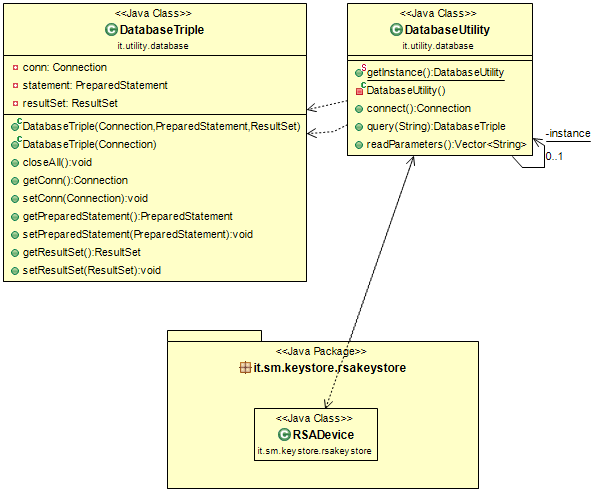
\includegraphics[scale = .5]{img/dependencies_utility_database}
	\caption{Package utility.database}
	\label{gfx:dependencies_utilitydatabase}
\end{figure}

\subsubsection{Package: \textbf{utility.mail}}

Contiene la classe per l’interfacciamento al mail server.

Il package è visualizzato in figura \ref{gfx:dependencies_utilitymail}.

\begin{figure}[!htbp]
	\centering
	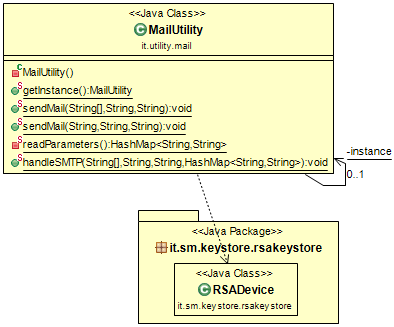
\includegraphics[scale = .5]{img/dependencies_utility_mail}
	\caption{Package utility.mail}
	\label{gfx:dependencies_utilitymail}
\end{figure}

\subsubsection{Package: \textbf{utility.network}}

Contiene la classe per l’interfacciamento al mail server.

Il package è visualizzato in figura \ref{gfx:dependencies_utility_network}.

\begin{figure}[!htbp]
	\centering
	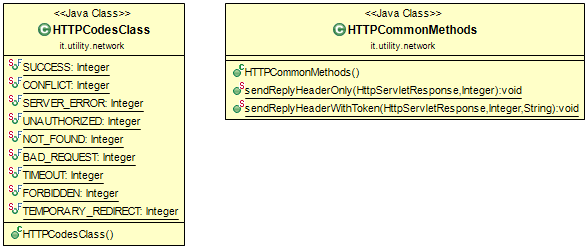
\includegraphics[scale = .5]{img/dependencies_utility_network}
	\caption{Package utility.network}
	\label{gfx:dependencies_utility_network}
\end{figure}

\subsubsection{Package: \textbf{webfilter}}

Le classi di questo package risolvono diversi problemi come il Cross Origin Resource Sharing.
Il package è visualizzato in figura \ref{gfx:dependencies_webfilter}.

\begin{figure}[!htbp]
	\centering
	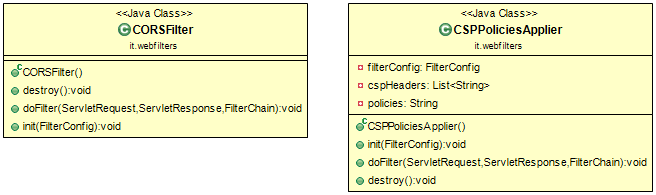
\includegraphics[scale = .5]{img/dependencies_webfilter}
	\caption{Package webfilter}
	\label{gfx:dependencies_webfilter}
\end{figure}


\subsubsection{Package: \textbf{websocket}}

Questo package contiene le classi per la gestione delle Web Socket.
In particolare, contiene classi che consentono l'interfacciamento con il server nodeJS e la comunicazione dei dati relativi agli utenti che hanno correttamente effettuato la procedura di login.\\
Infatti, nel momento in cui un utente effettua il login presso il server principale, le sue informazioni saranno inoltrate anche al server nodeJS: per evitare la falsificazione delle informazioni che vengono inviate al server nodeJS, sono state predisposte alcune misure di sicurezza con cui il server nodeJS è in grado di capire se il messaggio ricevuto proviene effettivamente dal server principale o meno: per ulteriori dettagli, si rimanda ai sequence diagram relativi alla fase di login.\\

Il package è visualizzato in figura \ref{gfx:dependencies_websocket}.

\begin{figure}[!htbp]
	\centering
	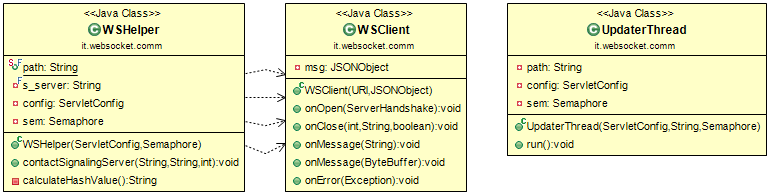
\includegraphics[scale = .5]{img/dependencies_websocket}
	\caption{Package websocket}
	\label{gfx:dependencies_websocket}
\end{figure}

\subsubsection{Package: \textbf{xml.registration}}

Il package è visualizzato in figura \ref{gfx:dependencies_xmlregistration}.

\begin{figure}[!htbp]
	\centering
	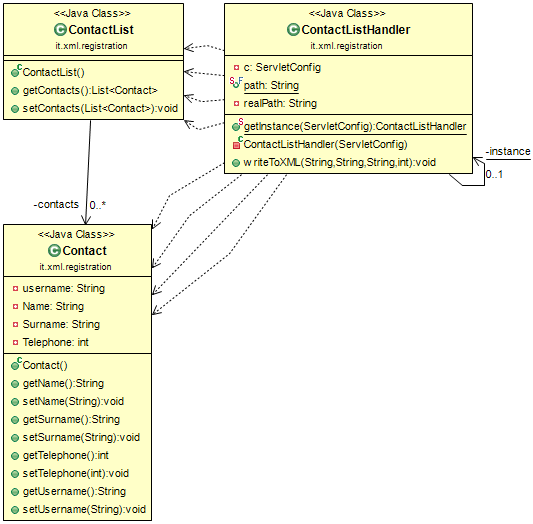
\includegraphics[scale = .5]{img/dependencies_xmlregistration}
	\caption{Package websocket}
	\label{gfx:dependencies_xmlregistration}
\end{figure}
%~~~~~~~~~~~~~~~~~~~~~~~~~~~~~~~~~~~~~~~~~~~~~~~~~~~~~~~~~~~~~~~~~~~~~
%    File      : webanalysis
%~~~~~~~~~~~~~~~~~~~~~~~~~~~~~~~~~~~~~~~~~~~~~~~~~~~~~~~~~~~~~~~~~~~~~

\textual
\newpage
%\chapter{Dependability}\label{cap:dependability}

\section{Sequence Diagrams}

In questa sezione vengono mostrati e commentati i sequence diagrams realizzati per le funzionalità più significative dell'applicazione realizzata.

\subsection{Scenario Login}

In figura \ref{gfx:sdlogin} è riportato lo scenario di Login, con le operazioni che il sistema effettua rispetto agli input inseriti dall'utente. Si nota che sulla base della risposta ricevuta dalla servlet viene visualizzato un differente messaggio di errore 

\begin{figure}[!htbp]
	\centering
	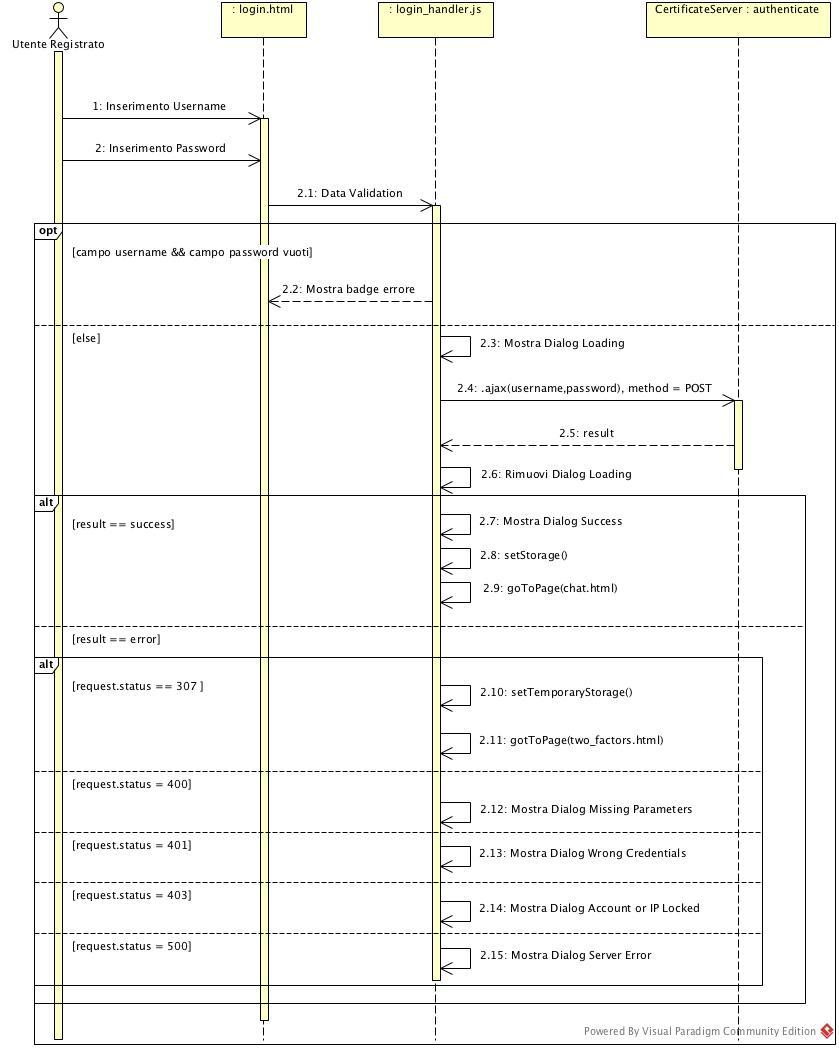
\includegraphics[scale = .4]{img/sd_login.jpg}
	\caption{Scenario Login}
	\label{gfx:sdlogin}
\end{figure}

\subsection{Scenario Registrazione}

In figura \ref{gfx:sdregister} è riportato lo scenario di Registrazione per gli utenti, con le operazioni che il sistema effettua rispetto agli input inseriti dall'utente, verificanti la validità della password in termini di strongness, richiedendo un carattere maiuscolo, uno minuscolo e un numero per un totale di almeno 8 caratteri, e dell'email, rispetto al formato. Si nota che sulla base della risposta ricevuta dalla servlet viene visualizzato un differente messaggio di errore.

\begin{figure}[!htbp]
	\centering
	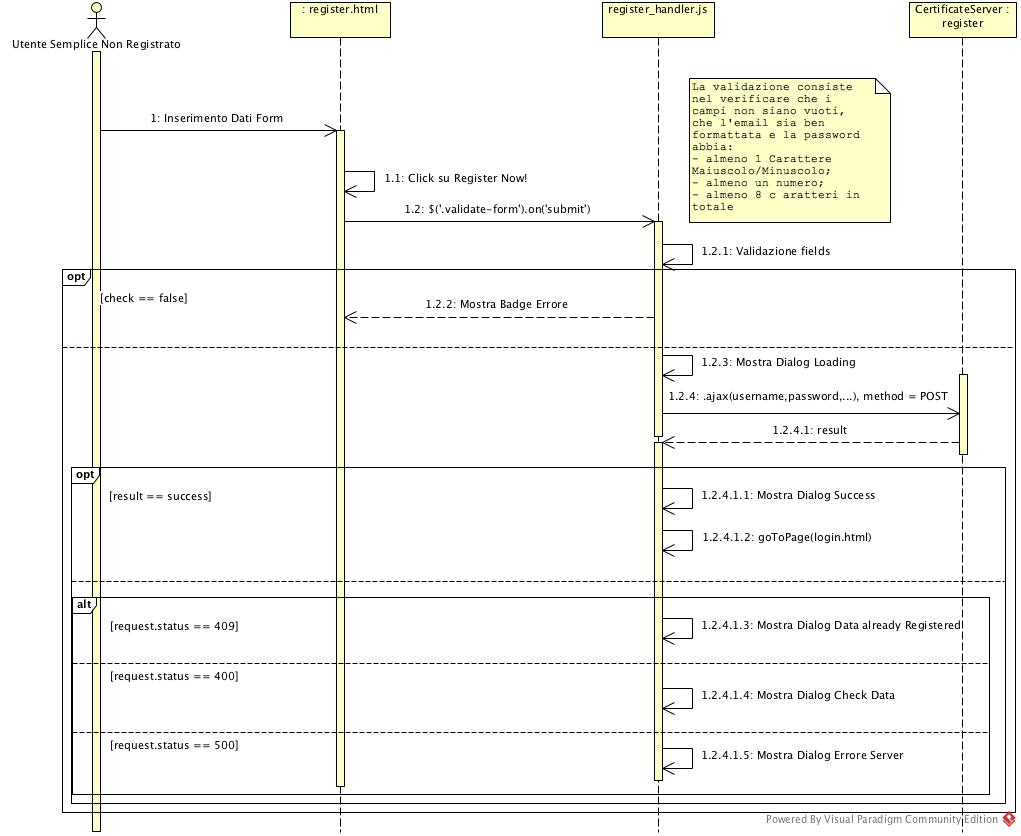
\includegraphics[scale = .4]{img/sd_register.jpg}
	\caption{Scenario Register}
	\label{gfx:sdregister}
\end{figure}

\subsection{Server Interaction (Login)}

In figura \ref{gfx:serverinteractionlogin} viene riportato il sequence diagram che descrive l'interazione che avviene tra il server NodeJS e il server Tomcat all'atto del login.

\begin{landscape}
\begin{center}

\begin{figure}[!htbp]
	\centering
	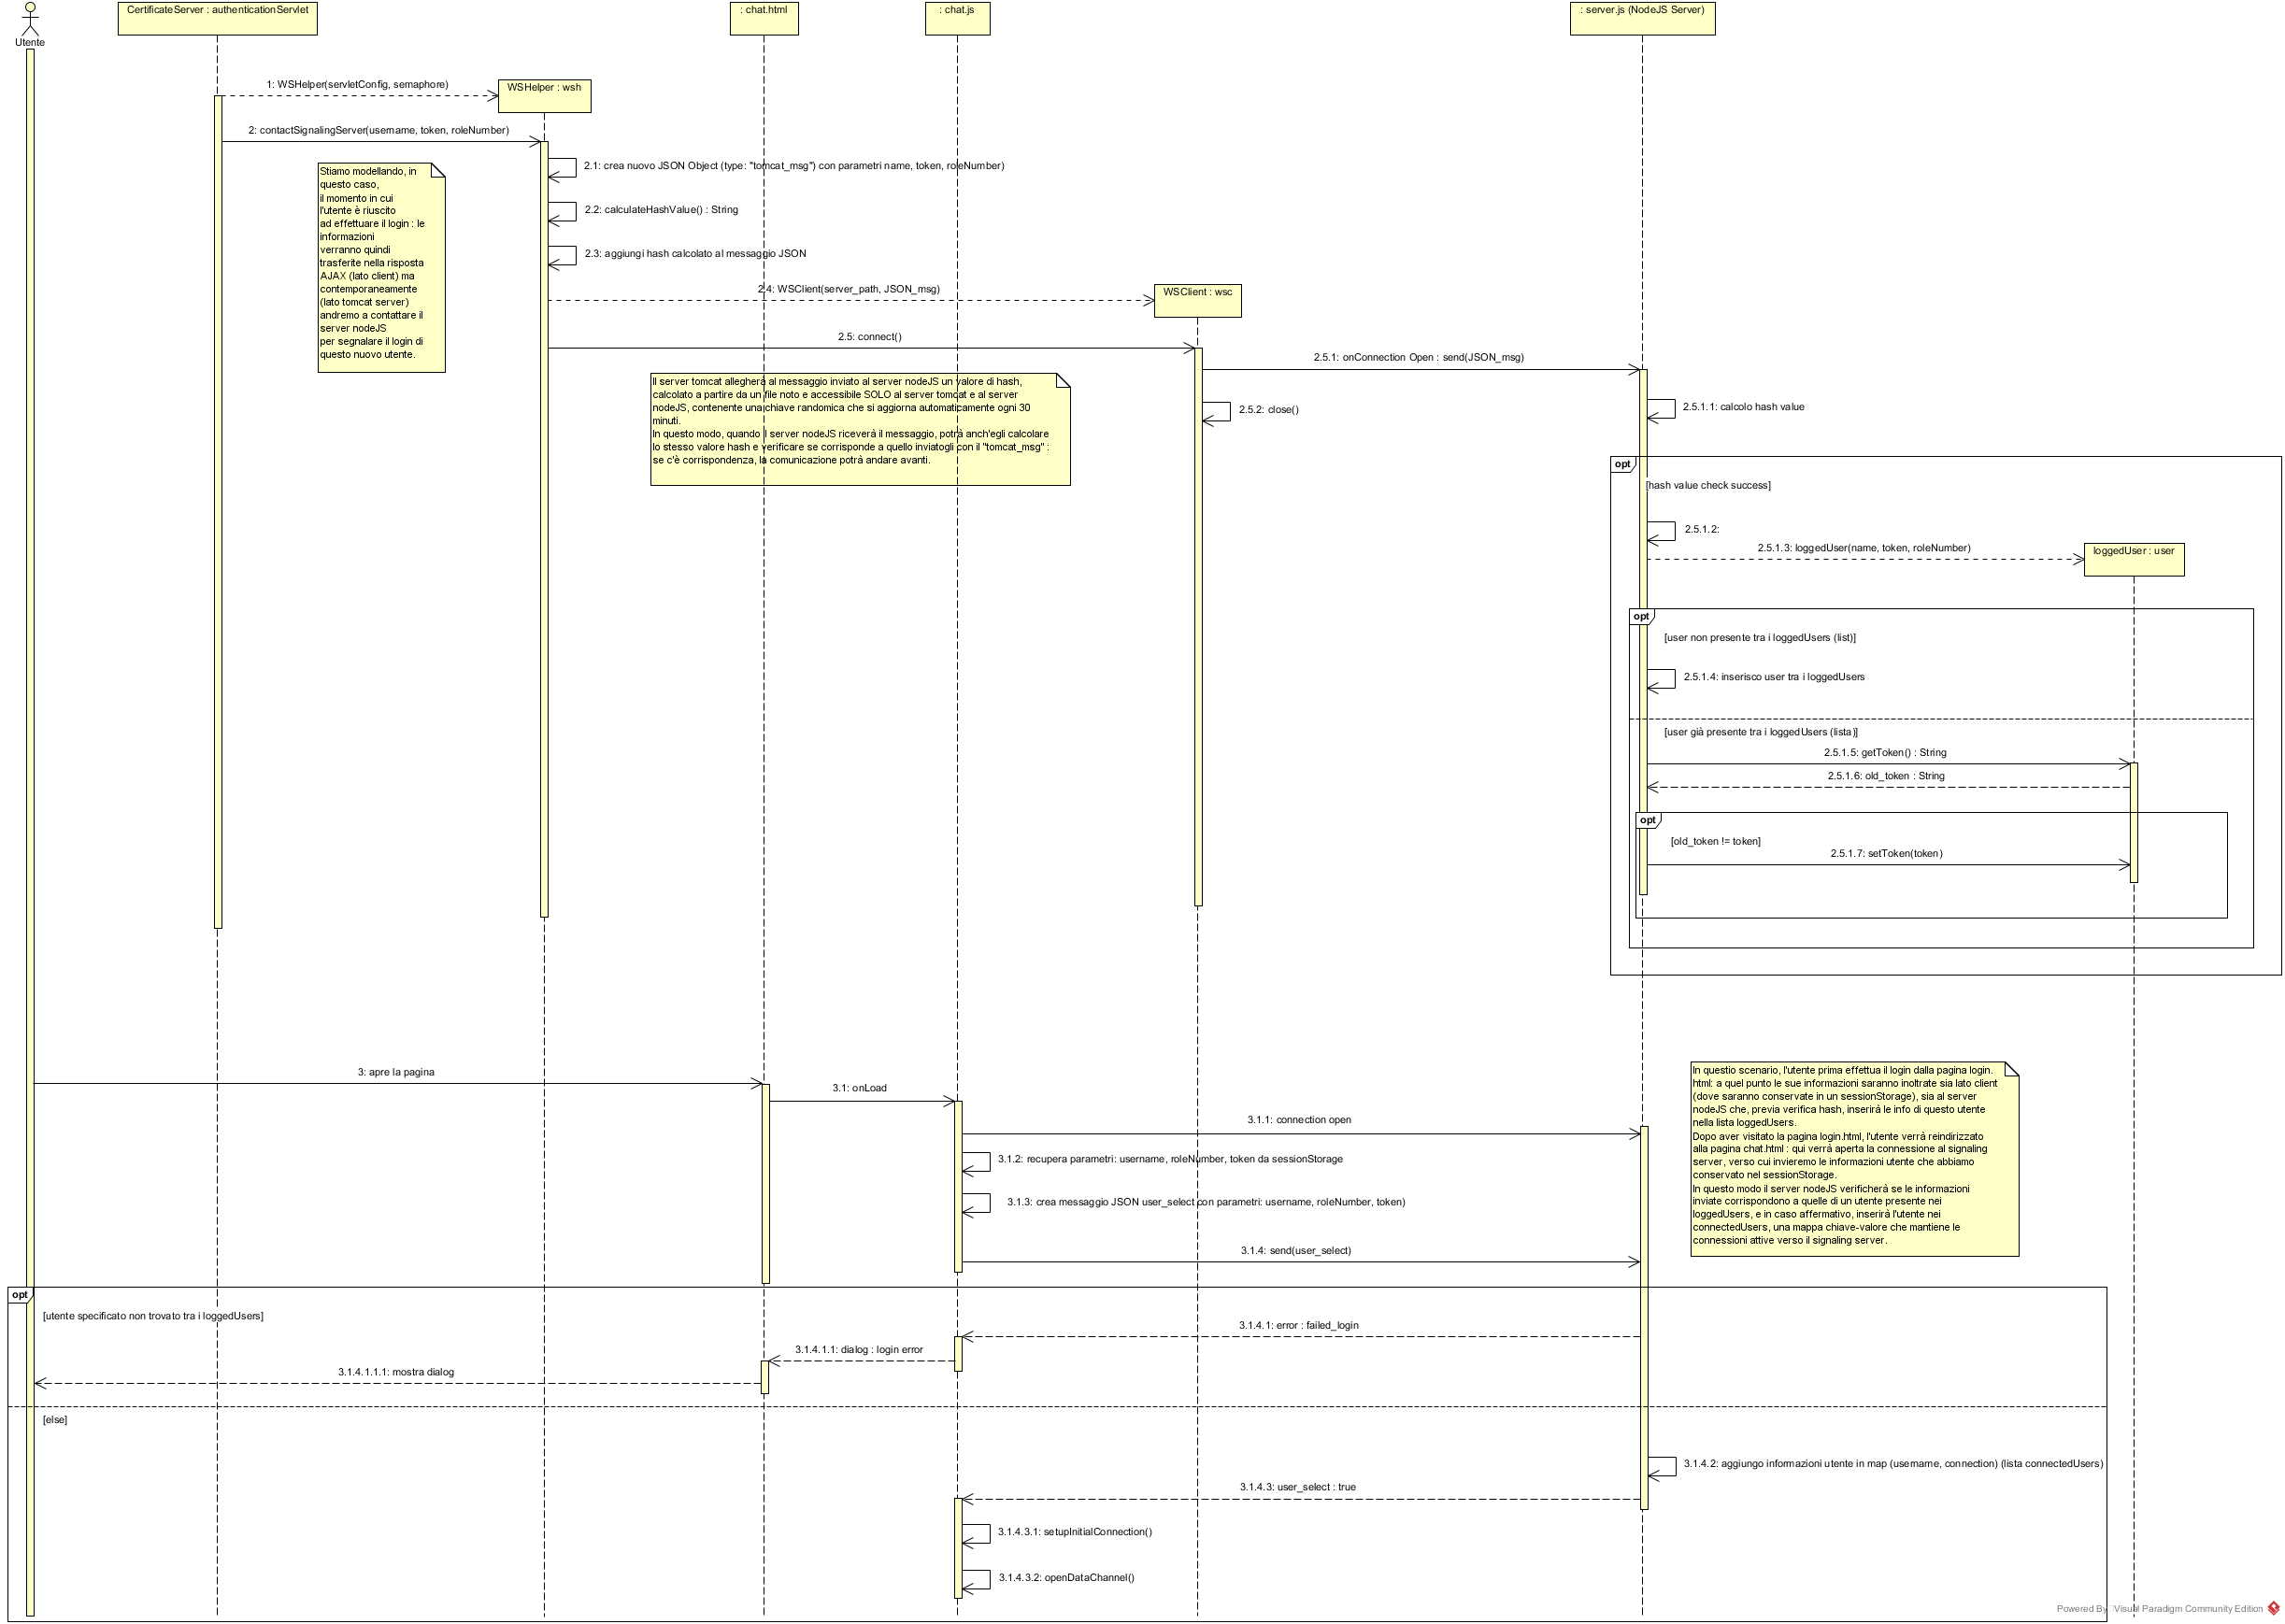
\includegraphics[scale = .31]{img/sequence_serverint.png}
	\caption{Server Interaction (Login)}
	\label{gfx:serverinteractionlogin}
\end{figure}
\end{center}	
\end{landscape}%

Quando un nuovo utente effettua correttamente il login presso la pagina login.html, accadono due cose:
\begin{itemize}
\item Le informazioni relative all'utente loggato vengono trasferite (come AJAX response) al client, che le conserva in un sessionStorage;
\item Il server Tomcat si occupa di contattare, mediante websocket, il server di segnalamento (nodeJS) per notificare il login di un nuovo utente.
\end{itemize}

Nel nostro caso, siamo interessati a modellare il secondo scenario.\\
Quando questo accade infatti, il server Tomcat aprirà una websocket verso il server nodeJS, passandogli le informazioni relative al nuovo utente loggato e, in aggiunta, un valore di hash: questo valore viene calcolato a partire da un file noto \textbf{esclusivamente} al server Tomcat e al server nodeJS (contenente una chiave randomica generata ogni 30 minuti): in questo modo, nel momento in cui il server nodeJS riceverà le informazioni sul login effettuato, potrà calcolare l'hash a partire dallo stesso file e verificarne la validità.\\
In caso di corrispondenza, il server nodeJS si occuperà di inserire l'utente specificato tra i cosiddetti \textit{loggedUsers}, ovvero coloro che hanno correttamente eseguito la procedura di login presso il server principale.\\
In questo modo, evitiamo che un qualsiasi utente possa contattare il server nodeJS e spacciarsi per un utente loggato.\\
Quando poi l'utente, accedendo alla pagina chat.html, si connetterà al signaling server (aprendo una websocket verso di esso), comunicherà a quest'ultimo le informazioni che ha ottenuto in fase di login (conservate nel sessionStorage) in modo che il server nodeJS potrà verificare se queste informazioni corrispondono effettivamente ad un utente presente tra i \textit{loggedUsers} (loggato correttamente): in caso affermativo, l'utente sarà inserito nei \textit{connectedUsers}, ovvero gli utenti con una connessione attiva verso il signaling server.\\
Per ulteriori dettagli si rimanda alla documentazione interna del server nodeJS.\\



\subsection{Offer Interaction}

In figura \ref{gfx:offerinteraction} si mostra l'interazione che si viene a realizzare ogniqualvolta un utente decide di inviare una \textit{offer} verso un altro utente, con l'intenzione di configurare e avviare una chat.

\begin{landscape}
\begin{center}
\begin{figure}[!htbp]
	\centering
	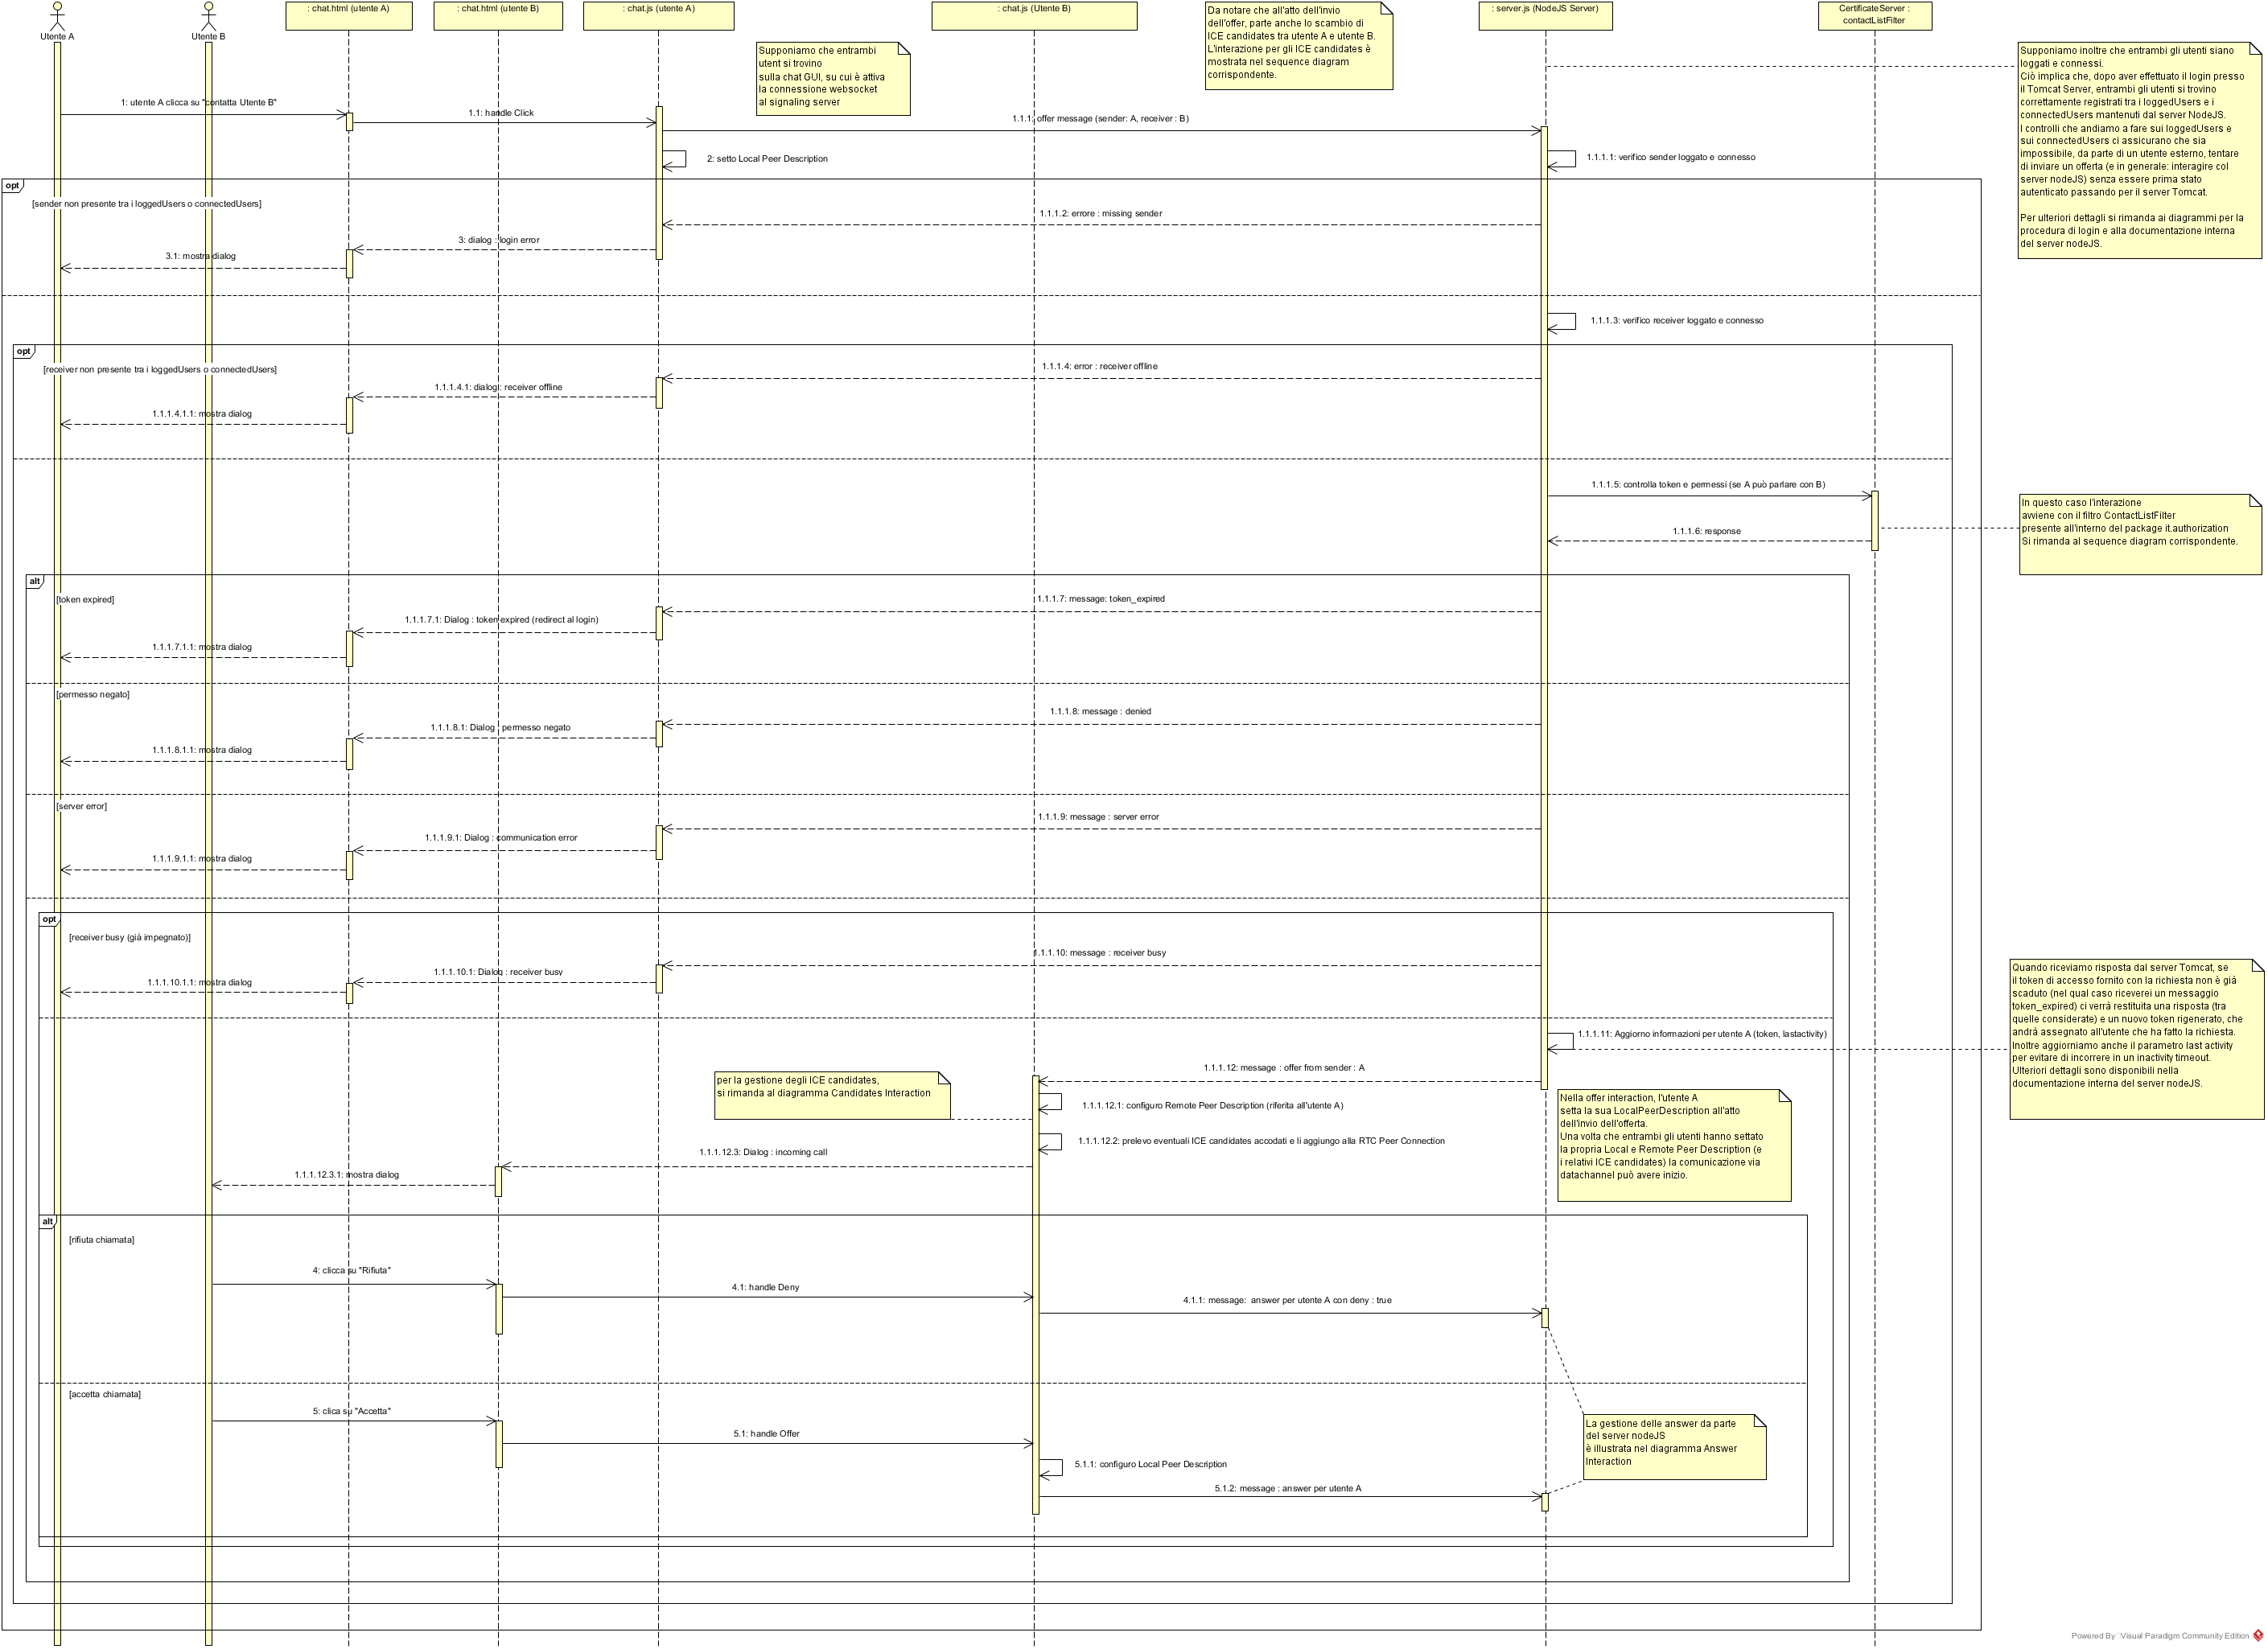
\includegraphics[scale = .25]{img/sequence_offer.png}
	\caption{Offer Interaction}
	\label{gfx:offerinteraction}
\end{figure}
\end{center}	
\end{landscape}%
Se supponiamo di avere un utente A che invia un messaggio offer destinato all'utente B, allora il server nodeJS, alla ricezione di tale messaggio, si occuperà di:
\begin{itemize}
\item verificare che l'utente A sia loggato e connesso (ovvero: presente tra loggedUsers e connectedUsers);
\item verificare che l'utente B sia loggato e connesso (ovvero: presente tra loggedUsers e connectedUsers);
\item verificare che l'access token di A sia valido;
\item verificare che A abbia il permesso di parlare con B (contattando il server tomcat e usando policy XACML);
\item verificare che B non sia già impegnato in un'altra chat.
\end{itemize}

Quando una di queste condizioni non dovesse essere verificata, il server nodeJS si occuperà di contattare il mittente (utente A) con un messaggio di stato opportuno.\\
Inoltre, se tutte le verifiche di cui sopra vanno a buon fine, il server nodeJS si occuperà di recapitare un messaggio offer verso l'utente B, che permetterà a quest'ultimo di configurare la comunicazione con l'utente A: in particolare, l'utente B potrà in questo modo configurare la sua \textit{LocalPeerDescription} (locale) e la \textit{RemotePeerDescription} (legata all'utente A, e ottenuta con le informazioni contenute nella offer).\\
Per ulteriori dettagli si rimanda alla documentazione interna del server nodeJS.\\


\subsection{Answer Interaction}

In figura \ref{gfx:answerinteraction} si riporta il sequence diagram che mostra l'interazione tra utente A e utente B nel momento in cui vi è l'invio di una \textit{answer}: supponendo che l'utente A voglia chiamare l'utente B, e che l'invio dell'offer sia avvenuto correttamente verso l'utente B, andremo a descrivere la comunicazione che avviene nel momento in cui B decide di inviare una answer ad A, tramite il signaling server.

\begin{landscape}
\begin{center}
\begin{figure}[!htbp]
	\centering
	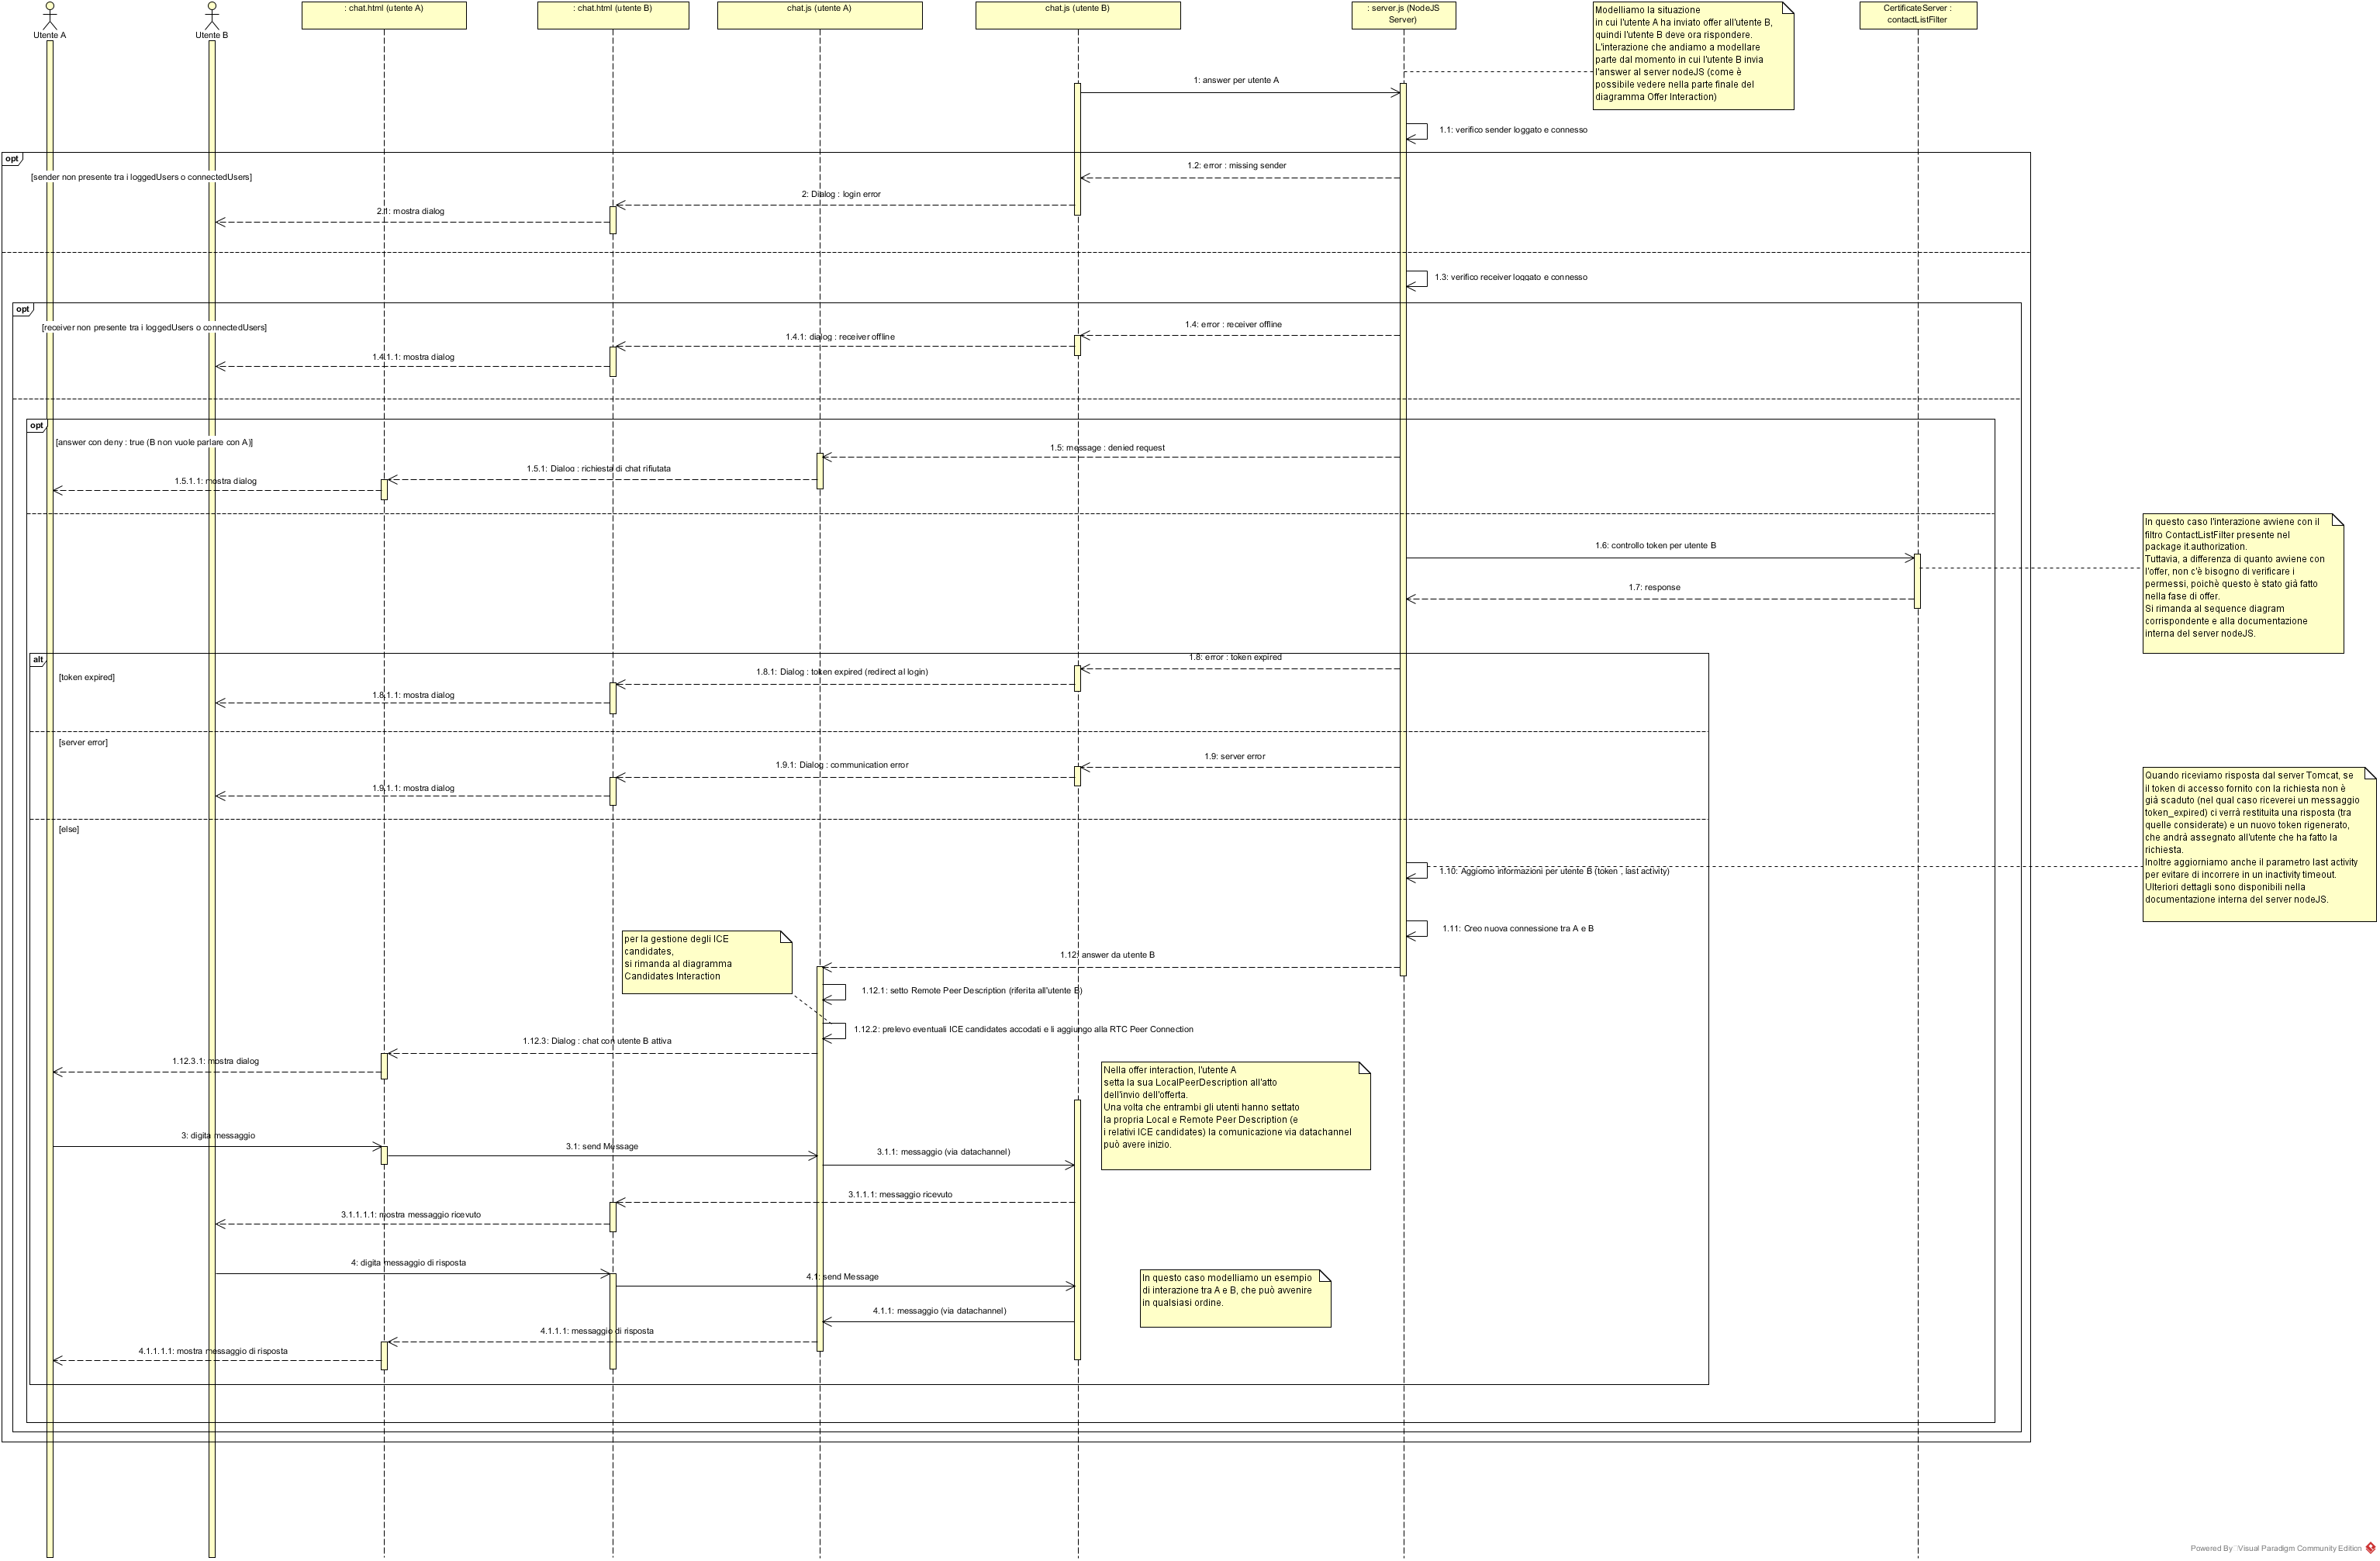
\includegraphics[scale = .26]{img/sequence_answer.png}
	\caption{Answer Interaction}
	\label{gfx:answerinteraction}
\end{figure}
\end{center}	
\end{landscape}%
Si nota che, in tal caso, quando l'utente B riceve l'offer da parte dell'utente A, si possono verificare due situazioni:
\begin{itemize}
\item l'utente B \textit{rifiuta} di parlare con l'utente A;
\item l'utente B \textit{accetta} di parlare con l'utente A.
\end{itemize}

Nel primo caso, l'utente B invierà al signaling server un messaggio answer contenente un campo \textit{deny}, con il quale il server nodeJS capirà che l'utente B ha rifiutato la chiamata e potrà quindi avvertire l'utente A di tale situazione.\\
Nel secondo caso, il server nodeJS riceverà un messaggio answer da parte dell'utente B, che dovrà poi essere recapitato ad A dopo aver verificato le stesse condizioni di prima.\\
In particolare, il server nodeJS si occuperà di:
\begin{itemize}
\item verificare che l'utente A sia loggato e connesso (ovvero: presente tra loggedUsers e connectedUsers)
\item verificare che l'utente B sia loggato e connesso (ovvero: presente tra loggedUsers e connectedUsers)
\item verificare che l'access token di B sia valido
\item verificare che l'utente B non abbia rifiutato di rispondere (in altri termini: se A chiama B, B può decidere di non rispondere)
\item verificare che A abbia il permesso di parlare con B (contattando il server tomcat e usando policy XACML)
\end{itemize}

Nel caso in cui una di queste condizioni non dovesse essere verificata, l'utente B (ed eventualmente l'utente A) saranno opportunamente avvertiti mediante appositi messaggi di stato.\\
Se invece la procedura va a buon fine, il signaling server si occuperà di inoltrare il messaggio di answer verso l'utente A: questo consentirà all'utente A di configurare sia la propria \textit{LocalPeerDescription} (locale ad A) sia la \textit{RemotePeerDescription} (legata all'utente B e ottenuta con le informazioni contenute nella answer).\\
In questo modo (una volta avvenuta anche la configurazione degli ICE candidates) la connessione è finalmente stabilita, e quindi utente A e utente B possono iniziare lo scambio di messaggi.\\
Per ulteriori dettagli si rimanda alla documentazione interna del server nodeJS.\\

\subsection{ICE Candidates Interaction}

In figura \ref{gfx:candidatesinteraction}, il sequence diagram illustra il meccanismo con cui avviene la comunicazione e lo scambio degli ICE candidates tra l'utente A e l'utente B.

\begin{figure}[!htbp]
	\centering
	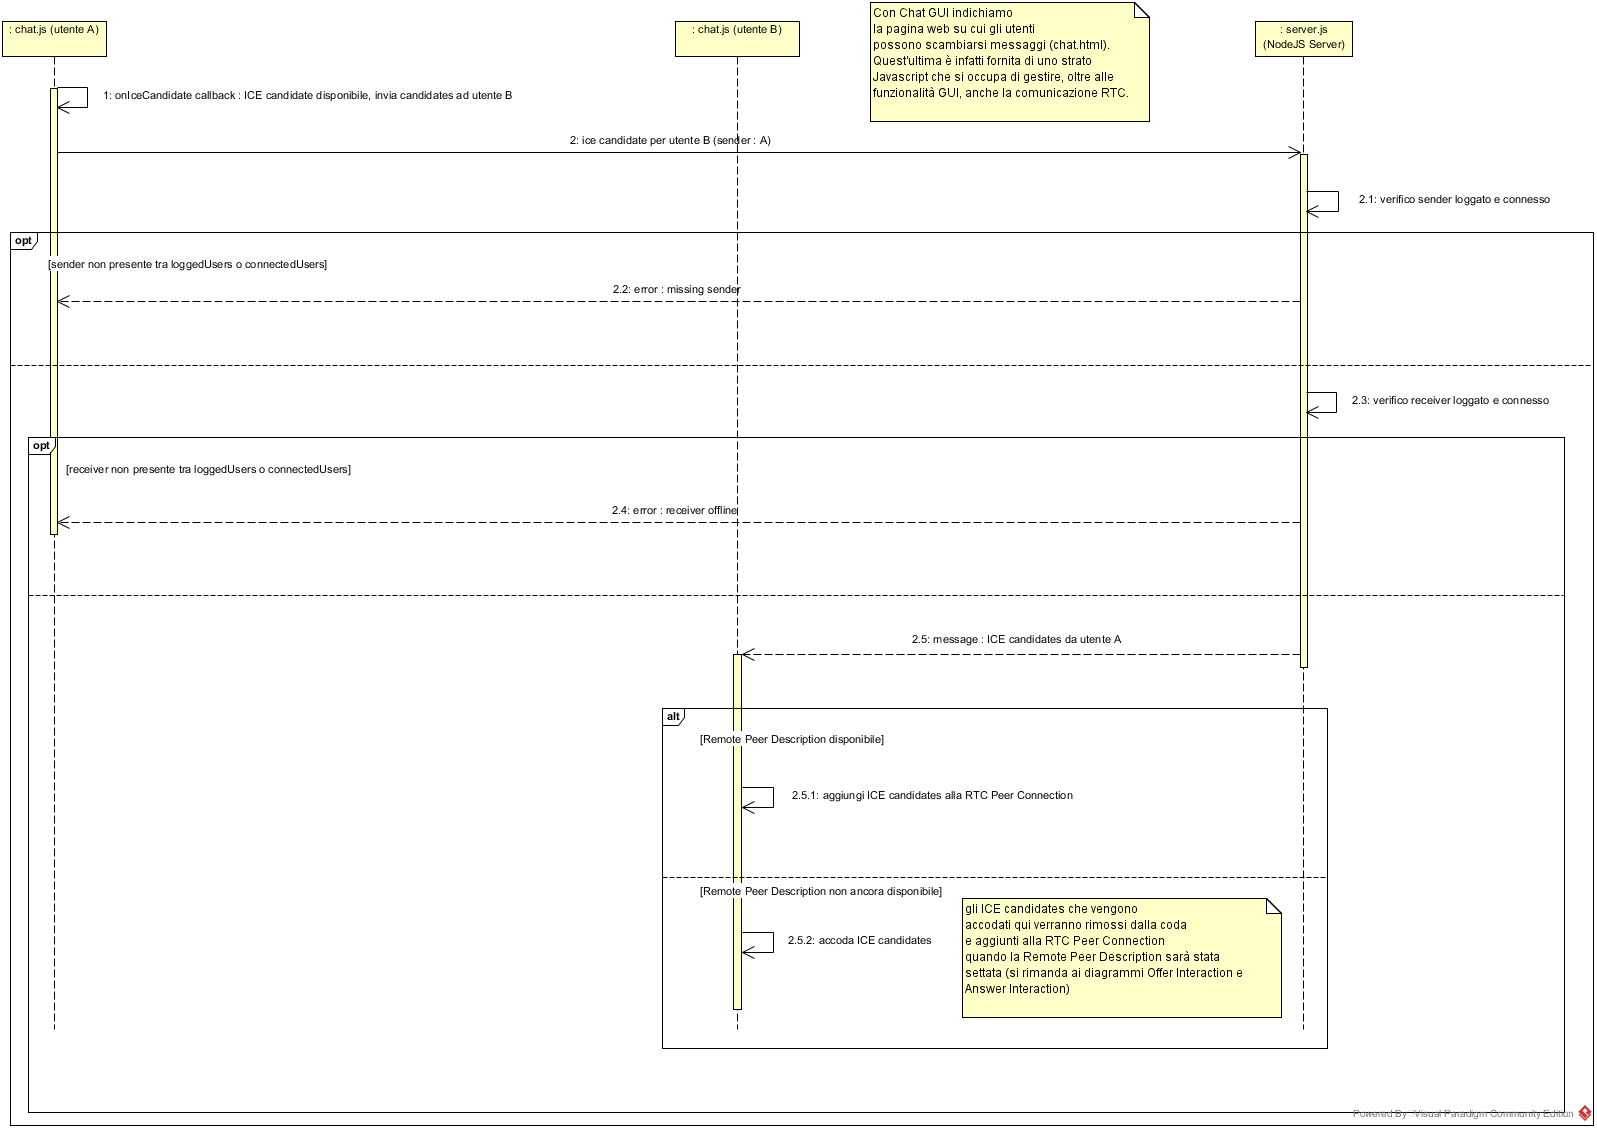
\includegraphics[scale = .37]{img/sequence_candidates.png}
	\caption{Candidates Interaction}
	\label{gfx:candidatesinteraction}
\end{figure}

Entrambi i client posseggono dei \textit{listener} per cui, non appena un ICE candidate risulta disponibile, viene inviato un messaggio verso il signaling server contenente informazioni a riguardo.\\
Il signaling server, dopo aver effettuato gli usuali controlli legati alla presenza degli utenti tra i \textit{loggedUsers} e i \textit{connectedUsers}, si occuperà semplicemente di inoltrare gli ICE candidates da un utente all'altro.\\
Tuttavia, visto che la configurazione degli ICE candidates può avvenire soltanto quando la RemotePeerDescription è stata settata, andremo ad accodare gli ICE candidates finchè non otterremo una RemotePeerDescription: a quel punto preleveremo i candidates dalla coda e configureremo di conseguenza la nostra connessione verso l'altro peer.\\
Ulteriori dettagli possono essere ottenuti osservando la documentazione interna del server nodeJS.\\

\subsubsection{Inactivity Timeout Interaction}

Il sequence diagram riportato di seguito mostra il meccanismo con cui è possibile rimuovere automaticamente un utente inattivo se quest'ultimo non effettua operazioni per più di un certo periodo di tempo.

\begin{figure}[!htpb]
	\centering
	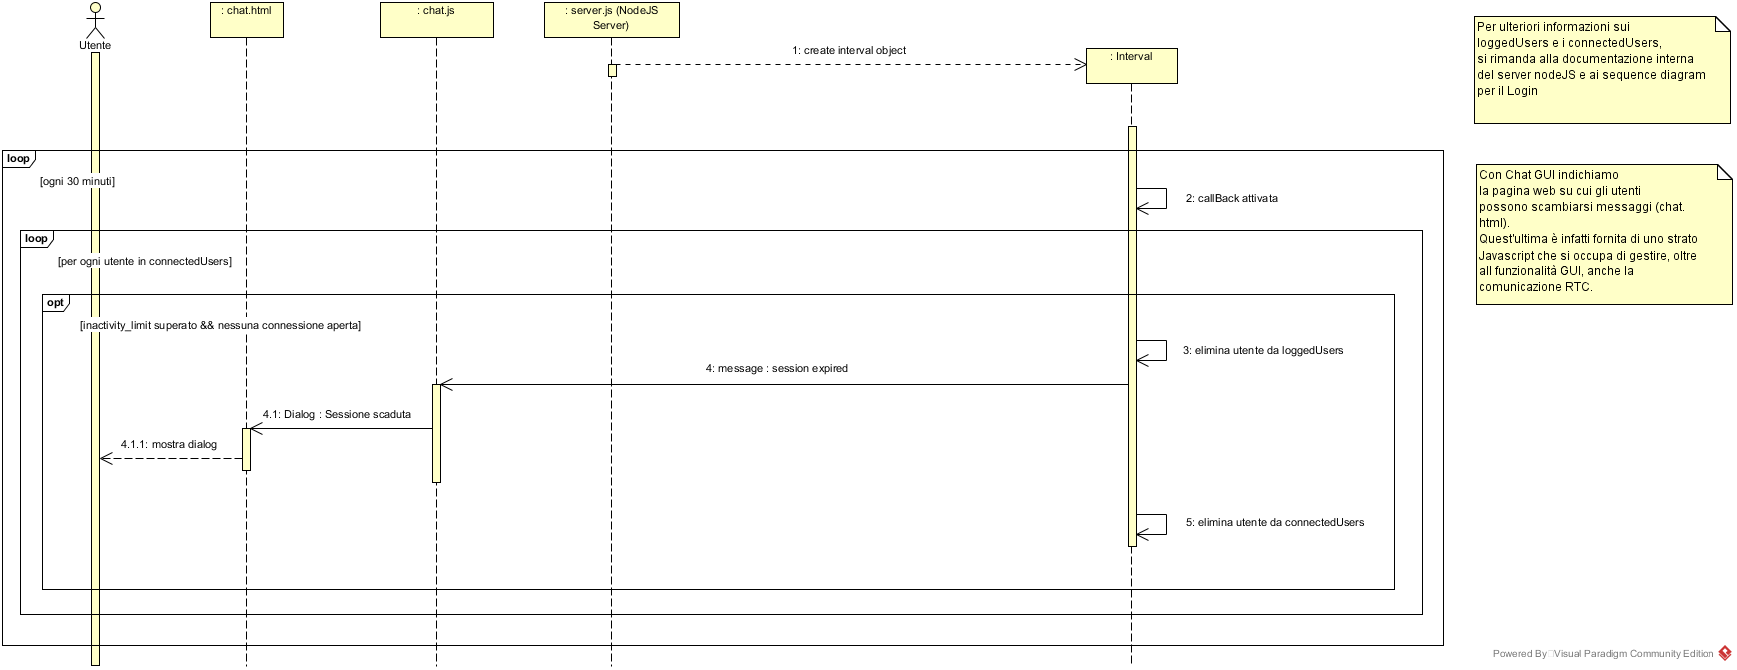
\includegraphics[scale = .35]{img/sequence_timeout.png}
	\caption{Timeout Inactivity Interaction}
	\label{gfx:timeoutinteraction}
\end{figure}

Il timeout è stato programmato per scattare ogni 5 minuti.\\
Quando la callback associata al timeout viene invocata, andremo ad analizzare tutti gli utenti con connessioni attive verso il signaling server (presenti tra i connectedUsers) per identificare quegli utenti che sono rimasti \textit{inattivi} (ovvero che non hanno inviato answer/offer e che non possiedono connessioni attive): tali utenti verranno quindi rimossi dai loggedUsers e dai connectedUsers, notificando l'evento con un apposito messaggio di stato lato client.\\

\subsection{Contact List Filter}

Il diagramma in figura \ref{gfx:contactlistfilter} mostra il comportamento del filtro ContactListFilter, utilizzato per l'accesso alle contact-lists che vengono prelevate dagli utenti ogni volta che si connettono alla chat, per poter selezionare (in base a policy ben precise) con quale utente comunicare.

\begin{figure}[!htbp]
		\centering
	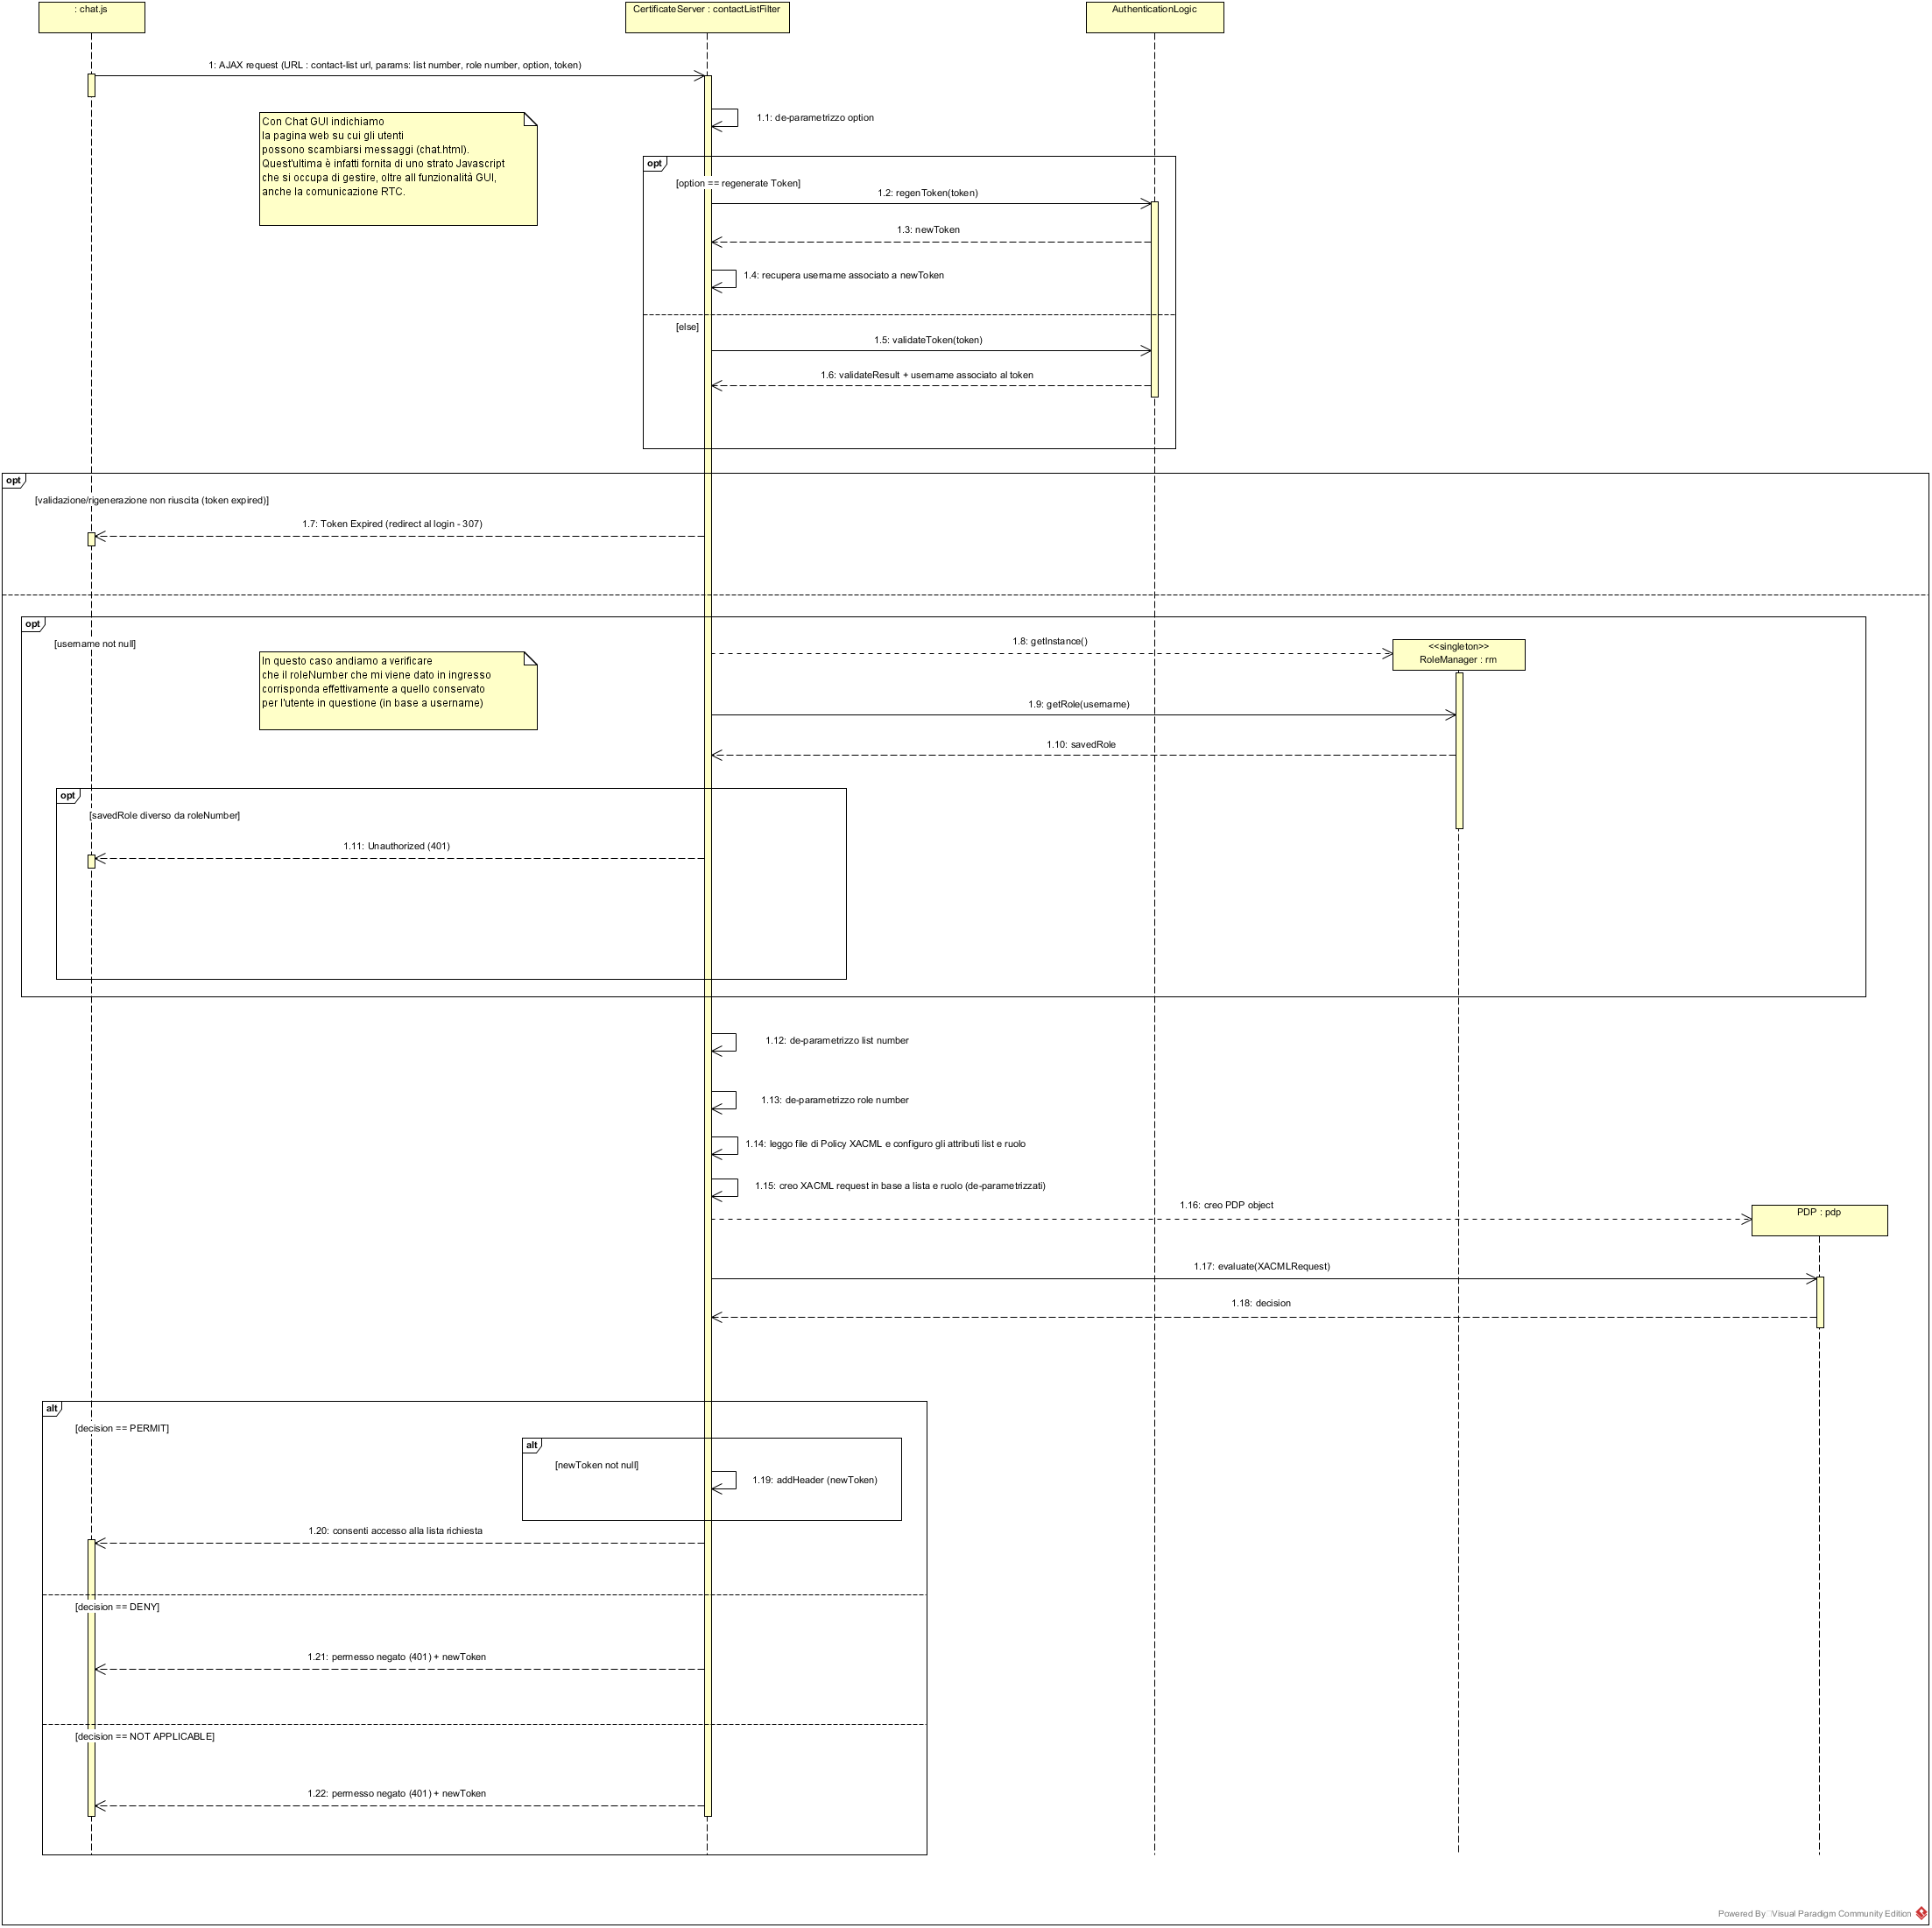
\includegraphics[scale = .26]{img/sequence_contactlist.png}
	\caption{Contact List Filter}
	\label{gfx:contactlistfilter}
\end{figure}
Il filtro viene attivato ogniqualvolta viene richiesto l'accesso al contenuto della cartella contact-lists, in accordo con quanto dichiarato nel file web.xml.\\
Le richieste contengono tipicamente i seguenti parametri (POST):
\begin{itemize}
\item list : lista a cui accedere
\item role : ruolo dell'utente richiedente
\item token: token di accesso
\item option : valore che indica rigenerazione/validazione del token
\end{itemize}
Alla ricezione della richiesta, verrà effettuata una de-parametrizzazione dei dati passati tramite POST (sfruttando una \textit{Integer Access Reference Map}, accessibile \href{https://static.javadoc.io/org.owasp.esapi/esapi/2.0.1/org/owasp/esapi/AccessReferenceMap.html}{qui}.\\
Dopodichè, andremo a verificare se è stata richiesta la rigenerazione del token o la sua semplice validazione: nel caso in cui il token dovesse essere scaduto, entrambe queste procedure falliranno: questo produrrà il sollevamento di un'eccezione con cui segnaleremo, lato client, un \textit{temporary redirect} (307) che reindirizzerà l'utente al login.\\
Una volta assicuratoci che il token di accesso è valido, andremo innanzitutto a verificare che il ruolo fornito dall'utente sia corrispondente al suo ruolo effettivo, dopodichè de-parametrizzeremo i dati che rappresentano lista e ruolo, per poi costruire la richiesta XACML che verrà sottoposta al PDP (\textit{Policy Decision Point}), previa lettura del file \textit{policy.xml} che contiene le XACML policies da applicare.\\
In caso di accesso consentito, il filtro si limita semplicemente ad allegare il token rinnovato (se presente) e a far avanzare correttamente la richiesta; in caso di permesso negato, invieremo comunque il token rinnovato (se presente), ma notificheremo il client con uno status code 401 (Unauthorized).\\

Per ulteriori dettagli, si rimanda alla documentazione interna del server nodeJS o del contact list filter.\\



          % ------------------------------------------------------------------------------
          % - PÓS-TEXTUAL
          % ------------------------------------------------------------------------------
          \postextual          
        

    \end{sloppypar}
\end{document}
